\startchapter{A one-dimensional model of scaling in Reverse Osmosis: ROSSpy}
\label{ROSSpy_chapter}

\section{Introduction}
Desalination technologies, most notably reverse osmosis (RO) \cite{Malaeb2011ReverseReview}, are imperative for meeting the 6th UN Sustainable Development Goal \cite{Jones2018TheOutlook} of universalizing potable freshwater. Arid Middle-Eastern countries, who are both relatively affluent and geographically prone to water scarcity, are embracing RO desalination to satisfy domestic water needs; Israel, for example, supplies $\frac{3}{4}$ of its domestic water from desalination \cite{Shemer2017SustainableImpact} and Saudi Arabia is responsible for $\approx 22\%$ of global water desalination \cite{Council2021WaterPrivatization}. RO is the most economical desalination technology \cite{Karime2008ROPlant,Hafez2003EconomicsStudy}, however, it remains insufficiently efficient and economical for the low-resource communities. RO efficiency can be improved \cite{Elimelech2011TheEnvironment,Semiat2008EnergyProcesses} a) with energy recovery devices \cite{Amy2017Membrane-basedProspects}, that allow RO to approach the thermodynamic limit of desalinating seawater \cite{Zarzo2018DesalinationFuture}, and b) by mitigating membrane fouling such as scaling \cite{Warsinger2015ScalingReview,Khan2013SourceSea,Tang2014FoulingPlant,Shmulevsky2017AnalysisMembranes}, where minerals deposit upon the membrane surface and decrease membrane permeability such that greater applied pressures and energy usage are required to maintain a permeate flux over time. Scaling occurs mechanistically either through homogeneous precipitation from the highly concentrated brine byproduct of RO \cite{VanWagner2009EffectPerformance,Belfer1998SurfaceMembranes} -- which is itself hazardous \cite{Fernandez-torquemada2012DispersionPlants,Clemens1955ToxicityWells,Allen1989ApparatusBrine,Munn1989EffectCrops} but can be processed into useful salts \cite{Allen1954ProcessBrine,Fenton1992DesalinationWells} in zero-liquid waste management systems \cite{Jeppesen2009MetalConcentrate,Mavukkandy2019BrineGeneration} or used in mixing-entropy batteries \cite{Ye2019Charge-FreeMaterials} -- or through heterogeneous deposition upon nucleation sites on the membrane surface \cite{Karabelas2014IncipientChannels,Warsinger2018InorganicOsmosis}. The heterogeneous mechanism specifically occurs in a hyper-concentrated layer adjacent to the membrane called the concentration polarization (CP)   \cite{McCutcheon2006InfluenceOsmosis,Murthy1997EstimationModel,Gruber2011ComputationalSystems,Sablani2001ConcentrationReview,Zydney1997StagnantSystems,Li2016Three-dimensionalChannel}, which is achieved as a consequence of the no-slip boundary condition -- analogous to the capillary effect -- that prevents the CP from mixing with the bulk solution since the velocity gradient of the fluid reaches zero adjacent to the stationary filtration membrane \cite{Rapp2017Fluids}. 

Scaling, unfortunately, is experimentally elusive \cite{Hu2014Real-timeSpectroscopy,Butt1995IdentificationAutopsy,Sheikholeslami2003KineticsM}. Computational programs \cite{Giere2009IsExperimentation,Wijmans1995TheReview} may supplement experimental procedures \cite{Lenhard2007ComputerModeling,Chai2007UltrasoundModules} as a means to investigate scaling and optimize RO efficiency; however, current programs are either unspecific to RO \cite{2018ZeroPHREEQC} or focus upon other aspects of RO: e.g. plant operation \cite{DesalitechROSASoftware,Chee2018PerformanceSoftware,SysCAD2020PHREEQCUnit,Bouchareb2019ExperimentalDesalination}, permeate flux \cite{Xu2012TOUGHREACT.0,Steefel2015ReactiveSimulation}, brine geochemistry \cite{Kundu2018TechnicalTechnology}, or fluid dynamics of the CP \cite{Walker2003AssessmentReaction}. Mathematical programs \cite{Radu2014ASystems,Karabelas2019PredictionSimulator} and some with a user interface \cite{SoftwareReverseOsmosis,Strubbe2018CalibrationFull-Scale} have been developed that simulate RO scaling, however, these lack an application programming interfaces (APIs), which is essential for the broad analyses, over a continuum of variables, that could accelerate geochemical scaling research. 

We therefore developed a unique one-dimensional model that captures both the geochemistry of scaling equilibria and the reactive transport of desalination, in contrast to existing one-dimensional RO models that utilize the steady-state approximation and the solution-diffusion model \cite{Strubbe2018CalibrationFull-Scale}. This one-dimensional RO model -- similar only to the WaterTap model \cite{NAWI2021WaterTap} -- is critically amenable with PHREEQC \cite{Parkhurst2015PhreeqcRM:PHREEQC,Charlton2011ModulesLanguages}, which provides a rigorous and open-source numerical implementation of our model, similar to previous studies of scaling \cite{Mitrouli2016CalciumExperiments,Warsinger2018InorganicOsmosis} and RO \cite{Bein1993OriginBrine,Wilson1993GeochemistryFormations,Casas2012SeawaterElectrodialysis,Yan2017ReverseVelocity}. We exemplify our model through replicating experimental literature and conducting numerous sensitivity analyses across continuums of parameter values. We further developed the only, to our knowledge, open-source API of RO reactive transport (ROSSpy: RO Scaling Software in Python) based upon our model, which fulfills identified needs of a scaling software for RO research \cite{Karabelas2020ScalingTools}, where users can create, execute, process, visualize, and export simulations with predicted scale mass per membrane filtration area ($\frac{g~scale}{filtration~m^2}$) and ionic brine concentrations. Developers are encouraged to contribute to ROSSpy, which we believe is an important stride towards satisfying research needs in scaling and ultimately reducing water insecurity, especially in low-resource contexts. 

\section{Methods}

\subsection{Conceptual}

Our model represents RO desalination as a one-dimensional reactive transport process along the membrane-solution interface. The feed is represented by the single-domain model in Figure S4, where the bulk and CP solutions are aggregated into a single solution, as opposed to the more resolved dual-domain model, where the bulk and CP solutions are distinguished (Figure S5) \cite{Chen2016AssessingModel,Scruggs2019TheInterface,Greskowiak2015AUVI,Mieles2012AnalyticalSystem}. The dual-domain remains elusive within the confines of PHREEQC code (Section 6 of the Supporting Information) and moreover we demonstrate that the single-domain model is sufficient to recapitulate experimental results. Our model represents feed at the RO inlet with the Dirichlet boundary condition \cite{Moes2006ImposingMethod,Bazilevs2007WeakMechanics} -- a mathematical description of constant conditions at a model boundary -- where the influent feed is assumed to be an infinite reservoir and thus its concentration is immutable. Our model represents the RO outlet with the Cauchy boundary condition \cite{Gosses2018ExplicitModels} -- a mathematical description of dynamic conditions at a model boundary -- where the effluent concentrations dynamically depend upon desalination. A glossary of parameters and variables for the equations and calculations are provided in Table S1.


\subsection{Numerical}
The geochemistry and reactive transport components of our RO model are numerically detailed in the following sub-sections. 

\subsubsection{Permeate Flux}
The permeate flux in our model is assumed to be 100\% water, similar to other RO models \cite{Li2012OptimalDesalination}, and it is calculated as the change in moles ($\Delta \Phi_{e}$) of feed solution in any examined cell $e$. Permeate flux is proportional to the difference between feed pressure $P$ and osmotic pressure $\pi$ \cite{VanWagner2009EffectPerformance,Schock1987MassModules,Lonsdale1965TransportMembranes}
\begin{equation} \label{pressure_differential}
    \Delta \Phi_{e} ~ \alpha ~ (P - \pi),
\end{equation} 
however, these pressures are not readily measured or reported; hence, we calculate the permeate flux via two comparable methods that are elaborated in the following sub-sections.

\paragraph{Method 1: Linear permeate flux}
One method assumes that permeate flux decreases linearly along the RO module. This causes the concentration -- which is represented by the concentration factor (CF) \cite{McCaffrey1987TheHalite.,Casas2012SeawaterElectrodialysis,Kartashevsky2015PhosphateEffluents,Yan2017ReverseVelocity,Evangelista1985APlants}
\begin{equation} \label{cf_definition}
    CF = \frac{initial}{final}~,
\end{equation}
as the quotient of initial to final ionic concentrations (influent vs. effluent), solution masses, or permeate moles \cite{Casas2012SeawaterElectrodialysis,Yan2017ReverseVelocity} -- to increase exponentially along the RO module. The negative slope of permeate flux is calculated between the first cell $1$ and the last cell $n$
\begin{equation} \label{flux_slope}
    slope = \frac{(\Delta \Phi_{n}-\Delta \Phi_{1})}{n}~,
\end{equation}
where the simulated membrane-solution interface is discretized into $n$ equal fractions (cells) of the total module length $l_{module}$. The permeate fluxes in these border cells, $\Delta \Phi_{1}$ and $\Delta \Phi_{n}$, are calculated through a system of equations. One of these equations
\begin{equation} \label{average_permeate_flux}
     \overbar{\Delta \Phi}_{e} = \frac{\Delta \Phi_{module}}{n} = \frac{\Delta \Phi_{n} + \Delta \Phi_{1}}{2}
\end{equation}
equates two definitions of the average permeate flux per cell $e$: 1) $\overbar{\Delta \Phi}_{e} = \frac{\Delta \Phi_{module}}{n}$ from the total permeate flux over the module $\Delta \Phi_{module}$, and 2) $\frac{\Delta \Phi_{n} + \Delta \Phi_{1}}{2}$, as the average between the border cells. The other equation is the definition of relative pressure loss over the RO module \cite{Srivathsan2014ReverseUnsteadiness,Gu2020ModelingNetworks} ($HL ; 0\le HL\le 1$) per \cref{pressure_differential},
\begin{equation} \label{head_loss}
     \Delta \Phi_{n}= \Delta \Phi_{1}*(1-HL),
\end{equation}
which is $\approx 10\%$ \cite{Fraidenraich2009ReverseExperiment,Evangelista1985APlants,Dandavati1975HollowSystems}. The substitution of \cref{head_loss} into \cref{average_permeate_flux} -- given $HL$, $\Delta \Phi_{module}$, and $n$ -- permits calculating $\Delta \Phi_{1}$ and  $\Delta \Phi_{n}$, the flux slope of \cref{flux_slope}, and subsequently $\Delta \Phi_{e}$ from a linear expression of permeate flux per module cell
\begin{equation} \label{intermediary_permeate_flux}
    \Delta \Phi_{e} = (slope*e+\Delta \Phi_{1}).
\end{equation}
% Our permeate efficiency parameter ($PE; 0<PE<1$) applies here as means of considering module inefficiencies like preexisting fouling in the RO module that lessen the permeate flux of the system. The $PE$ scalar attenuates the total module permeate flux over the module through reducing \cref{intermediary_permeate_flux}: i.e. $\Delta \Phi_{old~module} = \Delta \Phi_{new~module}*PE$; $PE=0$ leads to $\Delta \Phi_{e}=0 ~\forall~ e$; and $PE=HL=1$ leads to $\overbar{\Delta \Phi}_{e}=\Delta \Phi_{e} ~\forall~ e$.

The calculation sequence for this permeate flux method is summarized:
\begin{enumerate}
    \item Define $HL$, $\Delta \Phi_{module}$, and $n$
    \item Calculate the permeate flux slope [\cref{flux_slope,average_permeate_flux,head_loss}]
    \item Calculate the permeate flux in each cell $e$ [\cref{intermediary_permeate_flux}]
\end{enumerate}


\paragraph{Method 2: Linear Concentration Factor}
The second method of calculating the permeate flux assumes that the CF increases linearly, which causes the permeate flux to decrease non-linearly, along the RO module. The CF slope is calculated analogously to \cref{flux_slope}:
\begin{equation} \label{average_cf_slope}
    slope_{CF} =\frac{CF_{n}-CF_1}{n}.
\end{equation}
The effluent $CF_{n}$ is the average CF of all effluent ion concentrations 
\begin{equation} \label{cf_calculation_output}
    CF_{n}=\frac{\sum_{i=1}^j(C_{i,brine})}{\sum_{i=1}^j(C_{i,feed})},
\end{equation}
where $C_{i,brine}$ is the effluent concentration and $C_{i,feed}$ is the influent concentration of ion $i$, for all $j$ ions. Defining CF from \cref{cf_definition} in terms of moles of feed solution ($\Phi$, which is assumed to be 100\% water) reveals an equation 
\begin{equation} \label{cf_cell_definition}
    CF_e=\frac{\Phi_0}{\Phi_e}=\frac{\Phi_0}{\Phi_0-\Delta \Phi_{(1,e)}}
\end{equation}
that can calculate the moles of feed at the end of an arbitrary cell $e$ ($\Phi_e$), where $\Delta \Phi_{e} = \Phi_0 - \Delta \Phi_{(1,e)}$ and $\Delta \Phi_{(1,e)}$, as the sum of permeate flux that occurred between cell $1$ and the end of cell $e$, is separately the sum
\begin{equation} \label{moles_removed_to_cell}
    \Delta \Phi_{(1,e)}=\Delta \Phi_{e}+\Delta \Phi_{(1,e-1)}
\end{equation}
of permeate flux before the start of cell $e$ ($\Delta \Phi_{(1,e-1)}=\sum_{j=1}^{e-1}(\Delta \Phi_{j})$) and the permeate flux over cell $e$ ($\Delta \Phi_{e}$). The initial moles of feed $\Phi_0$ is calculated
\begin{equation} \label{feed_mass}
    \Phi_0=V_{feed}*MW_{H_2O}*\rho_{H_2O},
\end{equation}
from the volume of the feed channel $V_{feed}$, which is the product of the module length $l_{module}$ and the cross-sectional area of the feed channel $A_{feed}$
\begin{equation} \label{feed_area}
    A_{feed}=(A_{module}-A_{permeate})*\frac{th_{feed}}{th_{unit}}~,
\end{equation}
where $A_{module}$ and $A_{permeate}$ are the cross-sectional areas of the whole module and the permeate tube, respectively, and $th_{feed}$ and $th_{unit}$ are the thicknesses of the feed channel and the repeating membrane unit in Figure S1, respectively. The linear expression for $CF_e$ 
\begin{equation} \label{cf_permeate_flux}
    CF_e=(slope_{CF})*e+CF_{0}~,
\end{equation}
is then substituted into \cref{cf_cell_definition}, with the slope from \cref{average_cf_slope}, to yield an expression for the permeate flux (a negative change in feed moles) at the end of each examined cell $e$
\begin{equation} \label{moles_removal_per_cell} 
    -\Delta \Phi_{(1,e)}=\frac{\Phi_0}{((\frac{CF_{n}-CF_{0}}{n})*e+CF_{0})}-\Phi_0~,
\end{equation}
which can be substituted into \cref{moles_removed_to_cell} with the sum of previous permeate fluxes ($\Delta \Phi_{(1,e-1)}$) to yield the permeate flux over any examined cell $e$ ($\Delta \Phi_{e}$), analogously to \cref{intermediary_permeate_flux}. Note that $\Delta \Phi_{(1,e-1)}=0$ when $e=1$, since there are no previous cells. 

The calculation sequence for this permeate flux method is summarized:
\begin{enumerate}
    \item Define the effluent CF
    \item Calculate the feed capacity of the module [\cref{feed_mass,feed_area}]
    \item Calculate the CF slope [\cref{average_cf_slope}]
    \item Calculate the permeate flux in each cell [\cref{cf_cell_definition,moles_removed_to_cell,cf_permeate_flux,moles_removal_per_cell}]
\end{enumerate}

\paragraph{Comparison of permeate flux methods}
Scaling predictions from these two permeate flux methods are juxtaposed in Figure \ref{permeate_approach}. The most significant difference is observed at the mid-point of the simulated module ($0.47 m$), where the linear CF method predicts $0.99 \frac{gram}{m^2}$ of Gypsum scale while the linear permeate flux method predicts $0.0196 \frac{gram}{m^2}$ of Gypsum scale. The linear CF method subsequently predicts subtly less scale than the linear permeate method. These different distributions are explained by the dependency of scale upon the solution CF -- where the exponential increase in CF through the linear permeate flux method causes initially less, and then eventually more, scaling than the linear CF method -- however, the scale distribution ultimately equates between these two permeate flux methods to 3 significant digits: $38.7 \frac{gram}{m^2}$. These methods are therefore believed to only subtly affect the distribution, and not the total quantity, of scale within a module. Experimental literature is not known that can verify which method better reflects physical systems. 

\subsubsection{Geochemistry}
The geochemistry of RO scaling in our model is predicated upon the kinetic rate laws and thermodynamic equilibria that define each mineral dissolution and precipitation. These chemical processes are encapsulated in the PHREEQC databases that offer different a) geochemical models, b) permissible ranges of conditions, and c) sets of potential minerals to best represent a given system. These databases are complemented with the ChemW Python package that rigorously calculates the molecular mass of each mineral (see the ChemW PyPI documentation) to permit scaling predictions in the conventional units of $\frac{g~scale}{m^2~membrane}$.

\begin{figure}
    \centering
    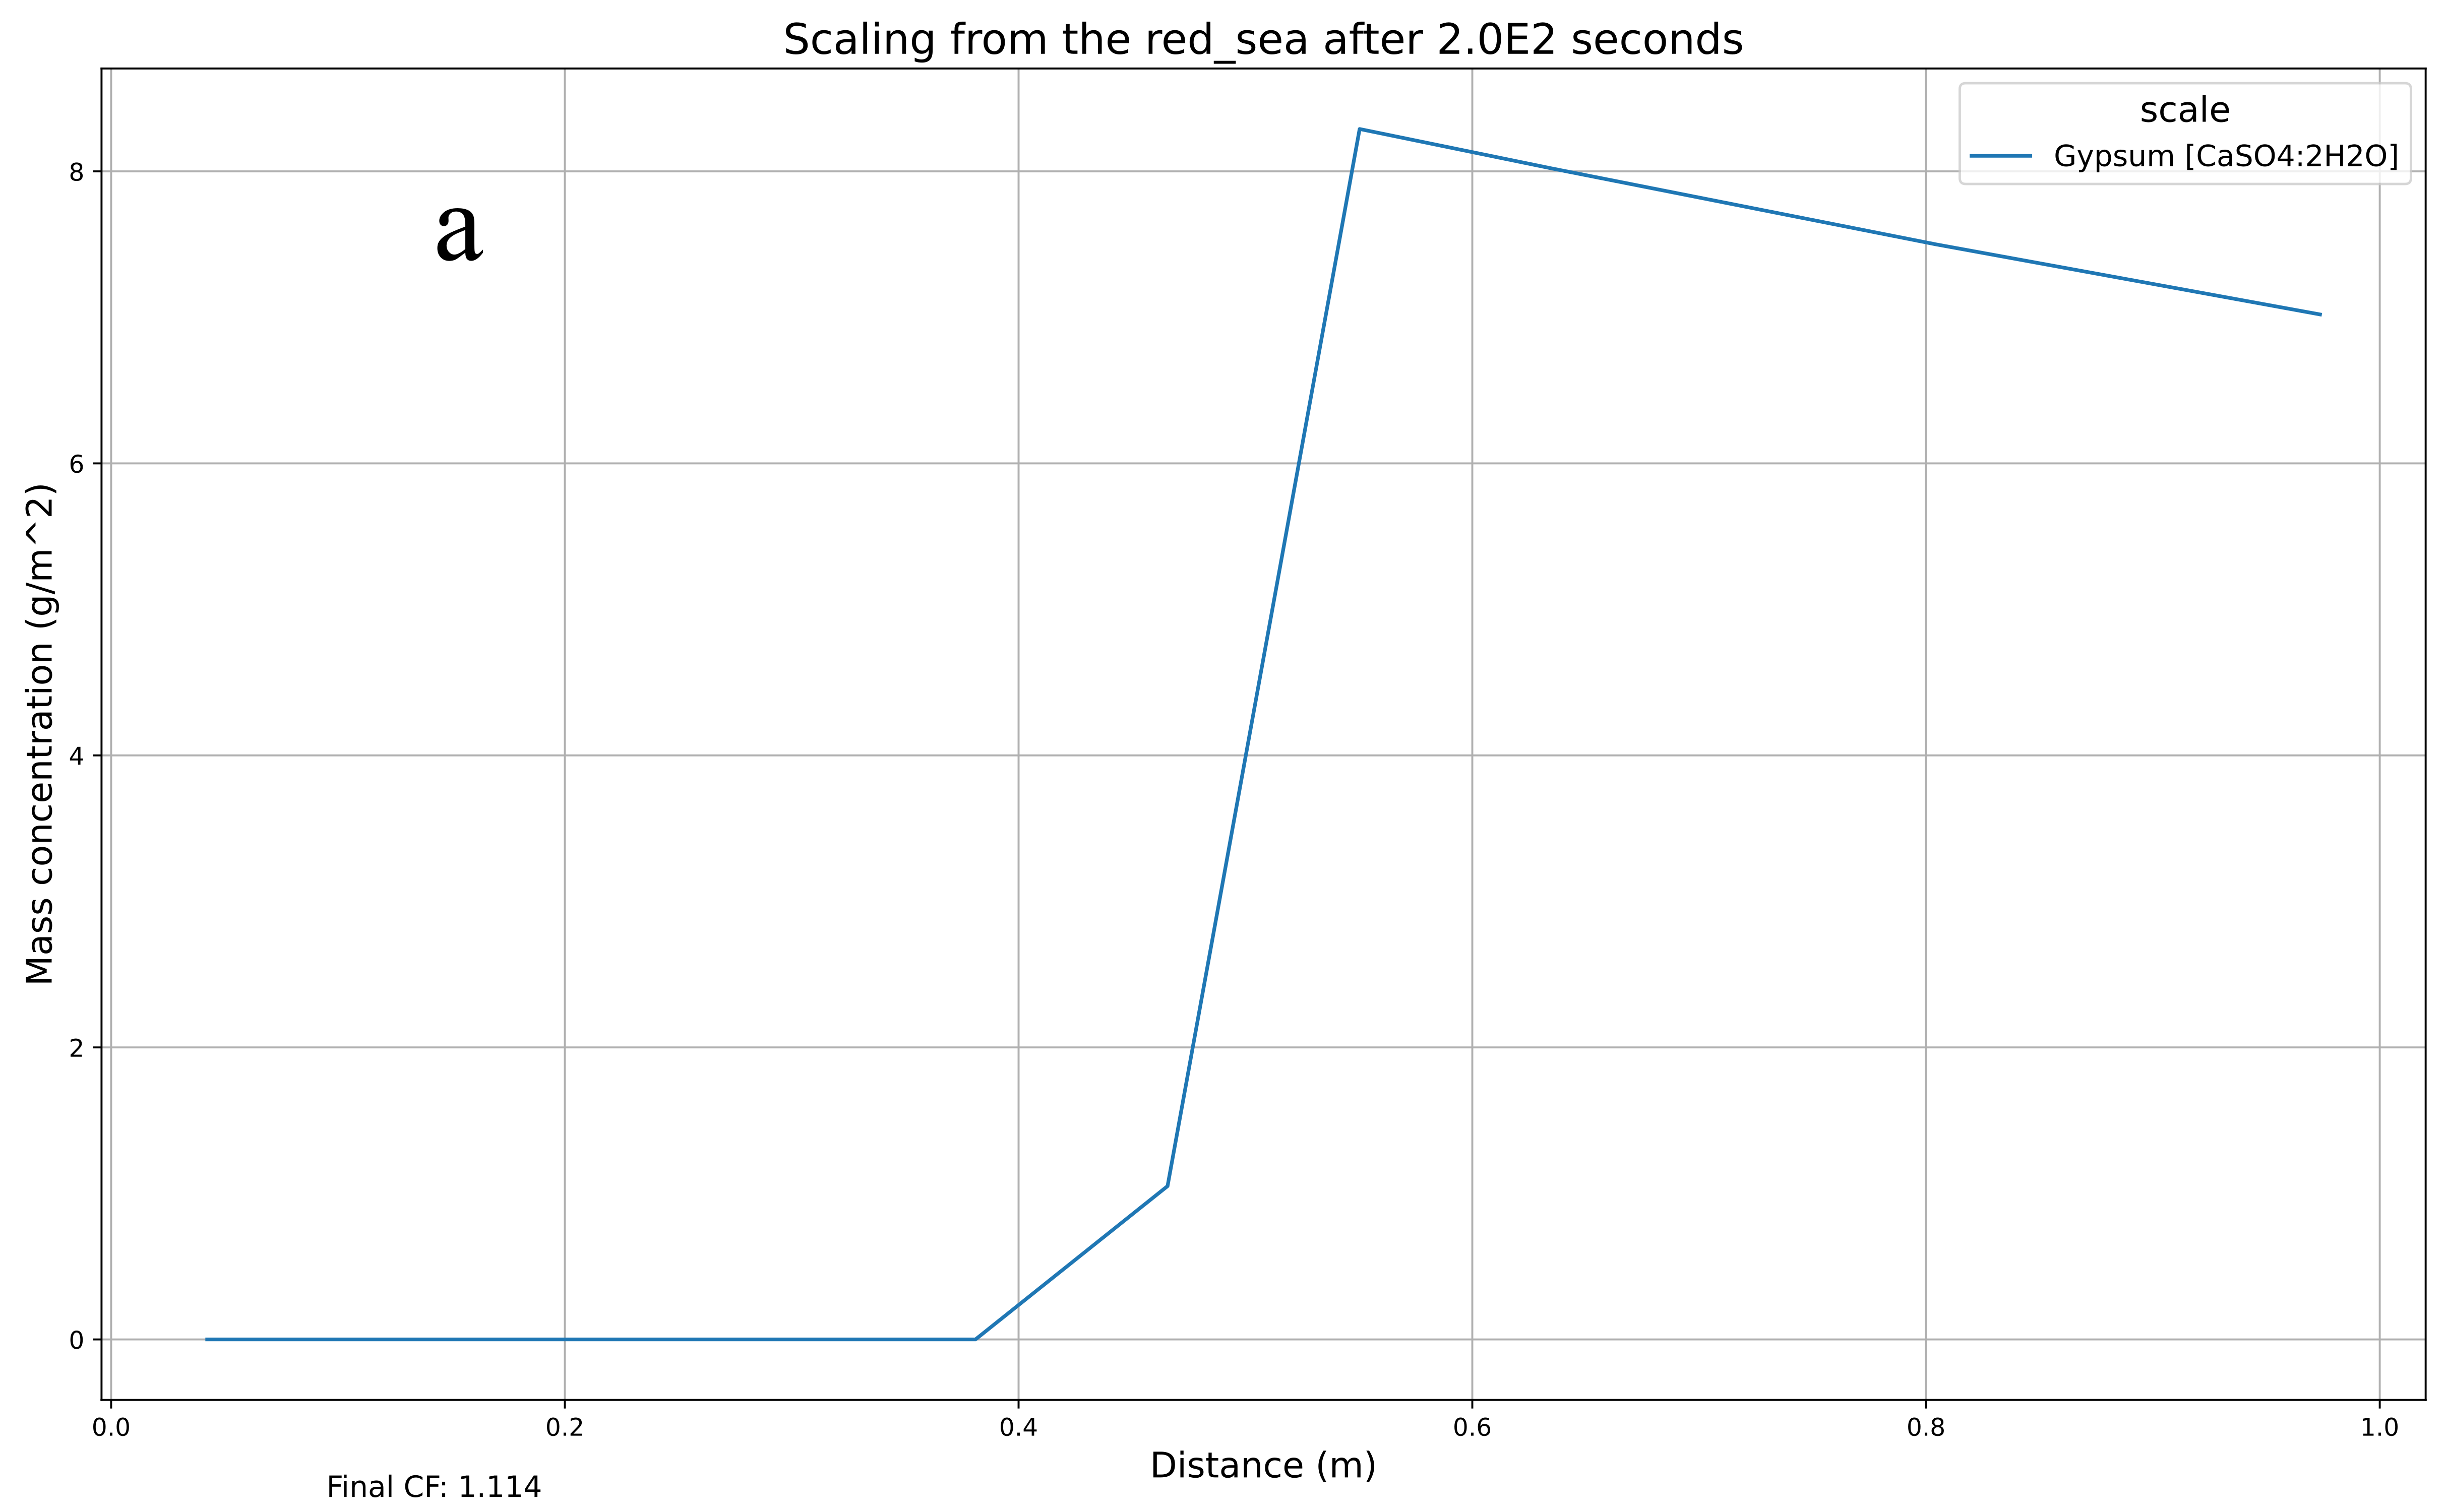
\includegraphics[width=0.9\linewidth]{images/ROSSpy/sensitivity_analyses/permeate_approach/linear_cf.png} \\ \midrule
    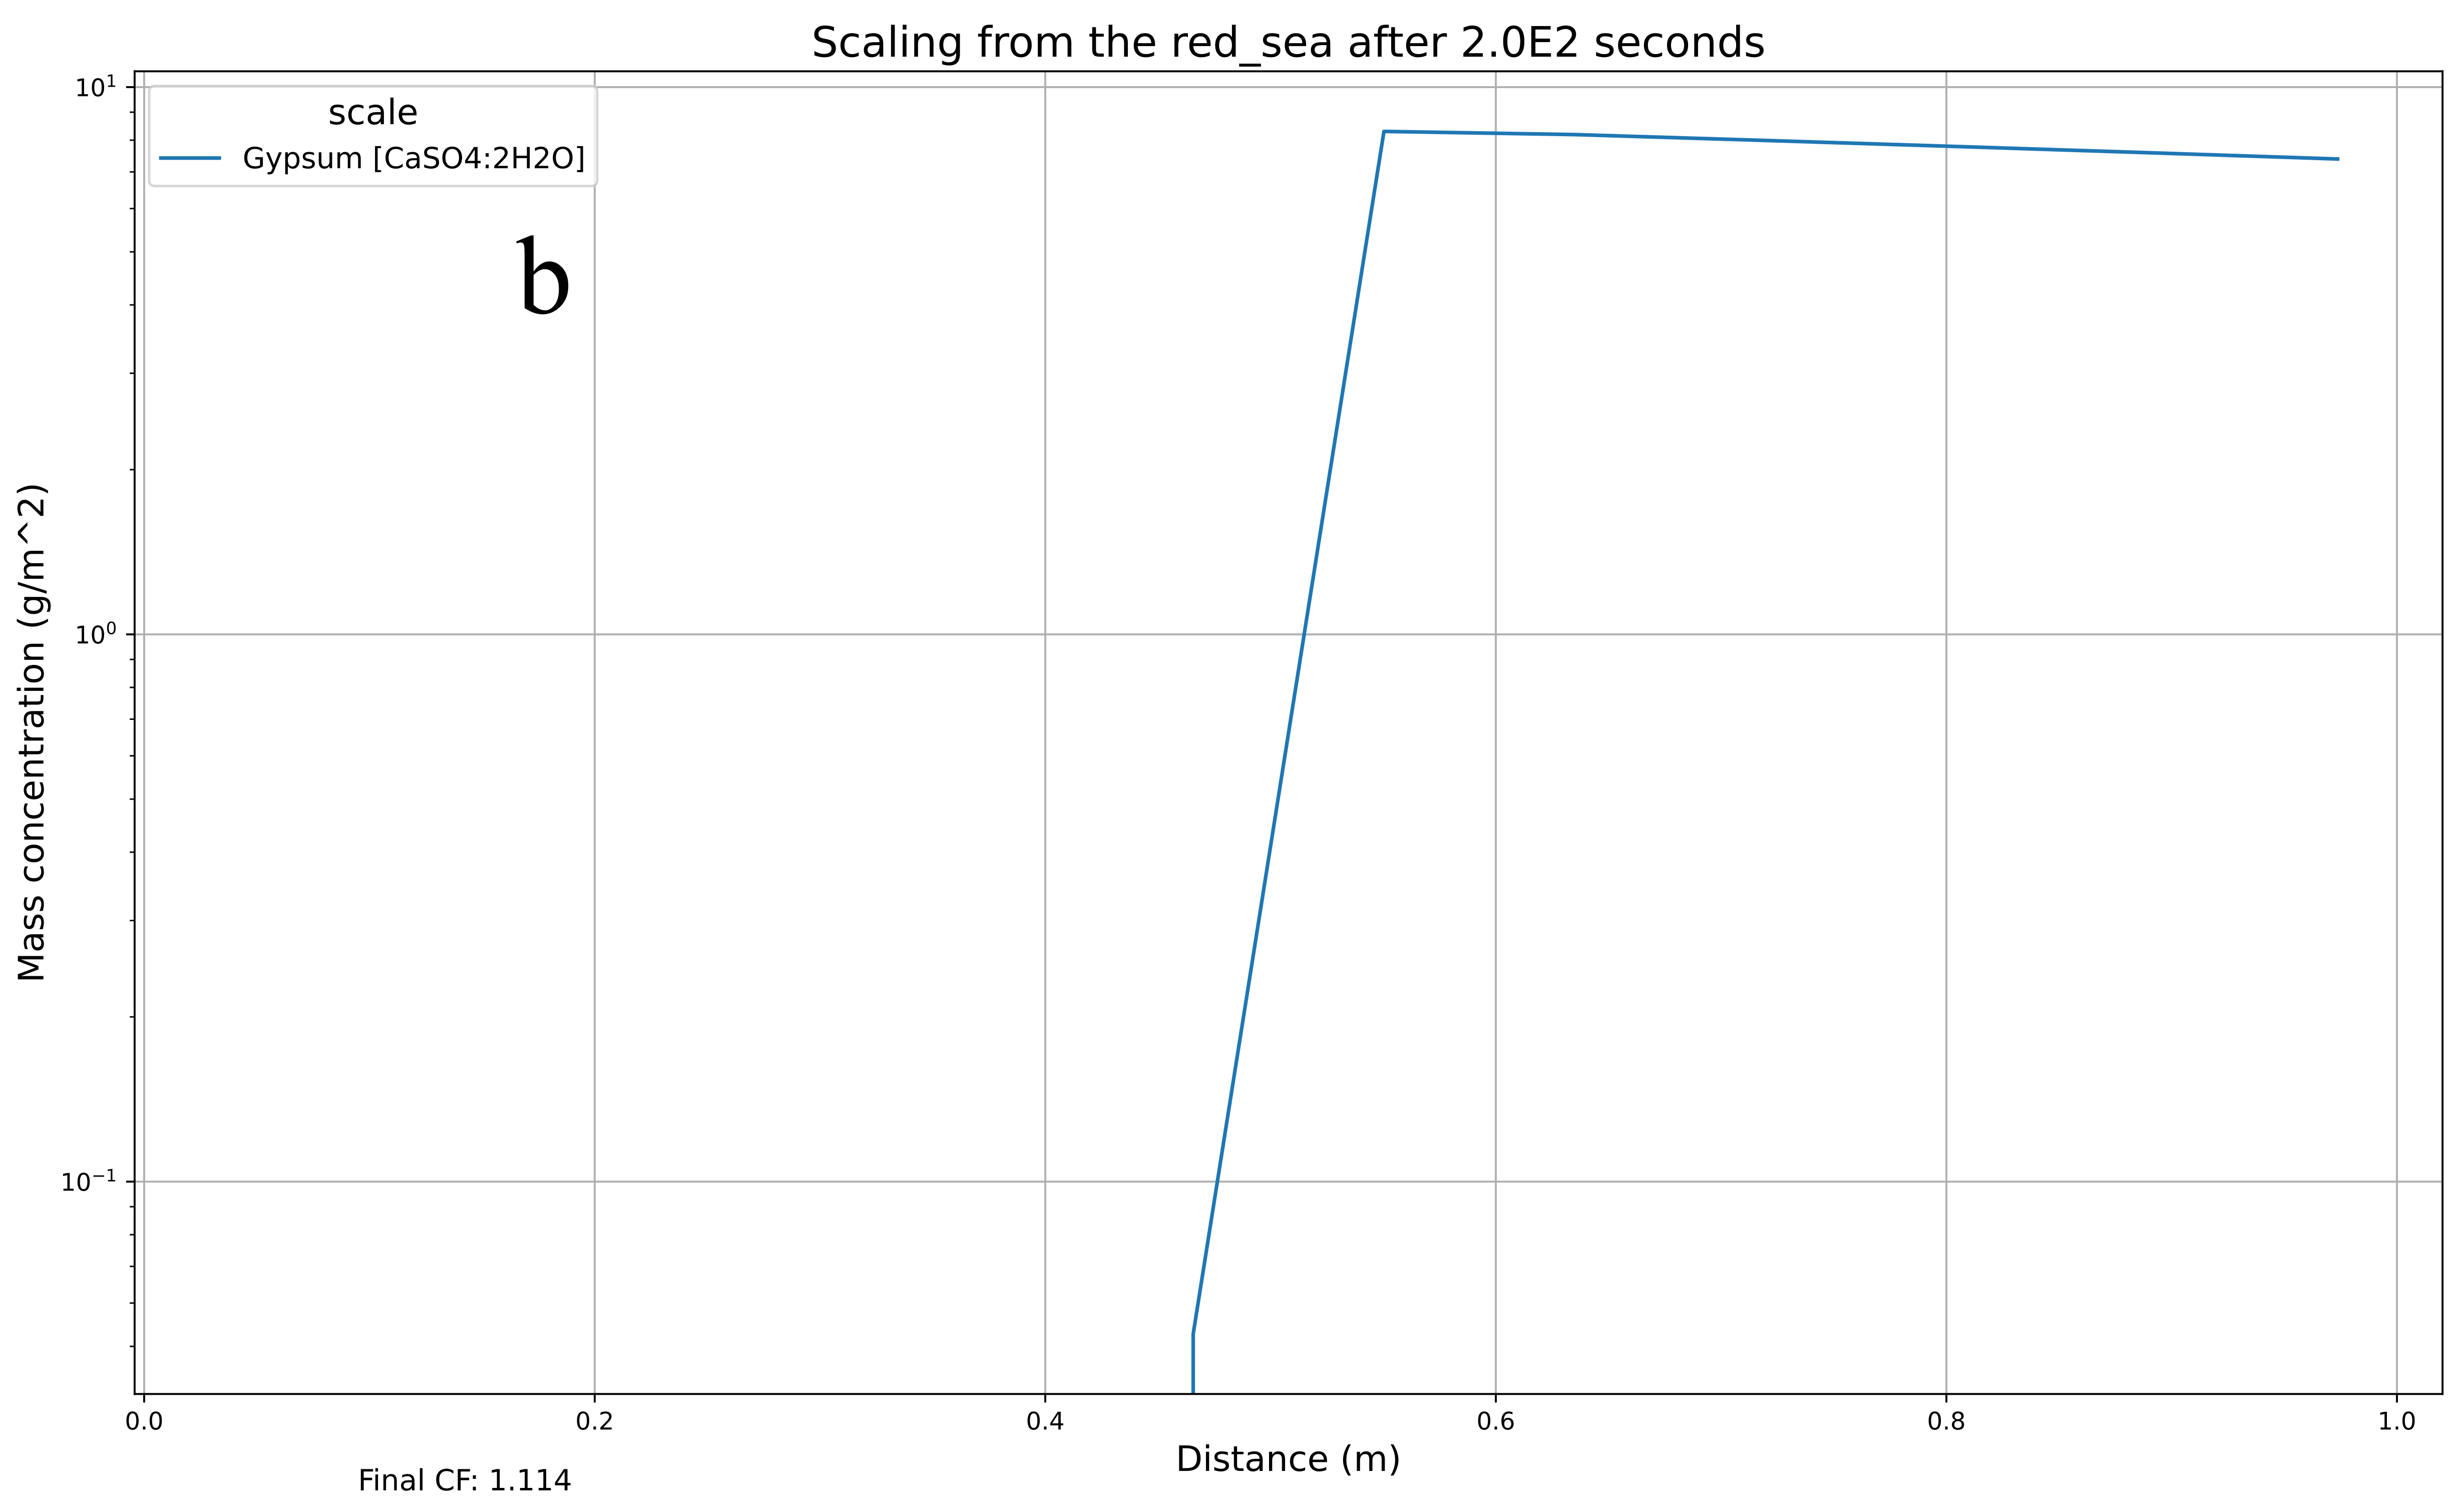
\includegraphics[width=0.9\linewidth]{images/ROSSpy/sensitivity_analyses/permeate_approach/linear_permeate.png} 
    \caption{
        Predicted scaling of the Red Sea at $CF_{effluent}=1.114$ via the a) linear CF and b) linear permeate flux methods. The linear increase in CF of a) slightly homogenizes the distribution of scaling, while the exponential increase in CF of b) skews the distribution of scaling to lesser initially and eventually greater, relative to the linear method of a). These subtle differences in scaling distribution neutralize as the total scaling through both methods are equivalent. 
    }
    \label{permeate_approach}
\end{figure}


\subsubsection{Transport}
The physical transport of feed through the module is simulated in each timestep by 1) migrating the contents of each cell $e$ to the next cell $e+1$; 2) repopulating cell $1$ as new feed solution enters the simulated module; and 3) deleting cell $n$ as brine exits the simulated module. The feed velocity $v_{feed}=\frac{Q_{max~feed}}{A_{feed}}$ is calculated from the maximum feed flowrate $Q_{max~feed}$ ($\frac{m^3}{s}$) and the feed area from \cref{feed_area} of the RO module. Default module parameters in Table S1 are sourced from the DOW FILMTEC BW30-400 RO module, similar to other RO models \cite{Li2012OptimalDesalination}, and supplement user-defined module parameters. The maximum simulation timestep $\Delta t=\frac{l_{cell}}{v_{feed}}$ is calculated according to the Courant Condition \cite{Gnedin2018EnforcingSchemes} ($C_{max}=1 \ge \frac{v_{feed}*t_{max}}{l_{cell}}$) to maintain accurate resolution of the feed flow.

\section{Use cases}
The following sub-sections evince features of our model and its alignment with reported measurements. These studies were conducted through ROSSpy and are available as Python Notebooks in the ROSSpy GitHub repository.

\subsection{CF and Brine formation}
The predicted CF and ionic concentrations of the effluent were verified through comparison with the following three experimental studies, where the reported feed geochemistry and module specifications were parameterized into the model. 

\paragraph{Zaman et al.\cite{Zaman2015DownstreamCompounds}}
This study examines RO brine, from a full-scale water treatment facility in Australia, to understand which minerals are likely to form as scale. The predicted concentrations in Figure \ref{bar_graphs}a were $<6\%-error$ for all but one of the feed ions.

\paragraph{Ahmed et al.\cite{Ahmed2001BrineEmirates}}
This study examines RO brine from 10 small desalination plants in Oman and 8 plants in the United Arab Emirates (UAE) for the purpose of understanding ideal brine disposal methods. We selected the UAE Qidfa I desalination plant from these 18 plants to replicate, since it provided the most comprehensive details. The predicted concentrations in Figure \ref{bar_graphs}b were $<10\%-error$ for all but one of the feed ions. The CF, in the far-right column of Figure \ref{bar_graphs}b, furthermore exhibits a $<1\%-error$, which supports that the reactive transport processes, notably the permeate flux calculations, are accurate.

\paragraph{Hajbi et al.\cite{Hajbi2010ReuseBrine}}
This study  evaluates the recovery of commodity salts from RO brine at a plant in Tunisia. The authors detail specifications of line D -- a polyamide filtration membrane -- in the plant system, in addition to the feed geochemistry, which were all parameterized into our model. The predicted concentrations in Figure \ref{bar_graphs}c were less aligned than the aforementioned two studies, with two ions exceeding $25\%-error$. This is attributed to $40\%$ fewer feed ions being defined by this study, where the incomplete geochemical representation of the feed skews the geochemical calculations of PHREEQC. This is corroborated by the accuracy of the CF prediction in Figure \ref{bar_graphs}c, despite inaccurate concentration predictions, which suggests that the error resides with the geochemical processes and not the reactive transport system. 

\begin{figure}
    \centering
    \begin{tabular}{c|c}
        \multicolumn{2}{c}{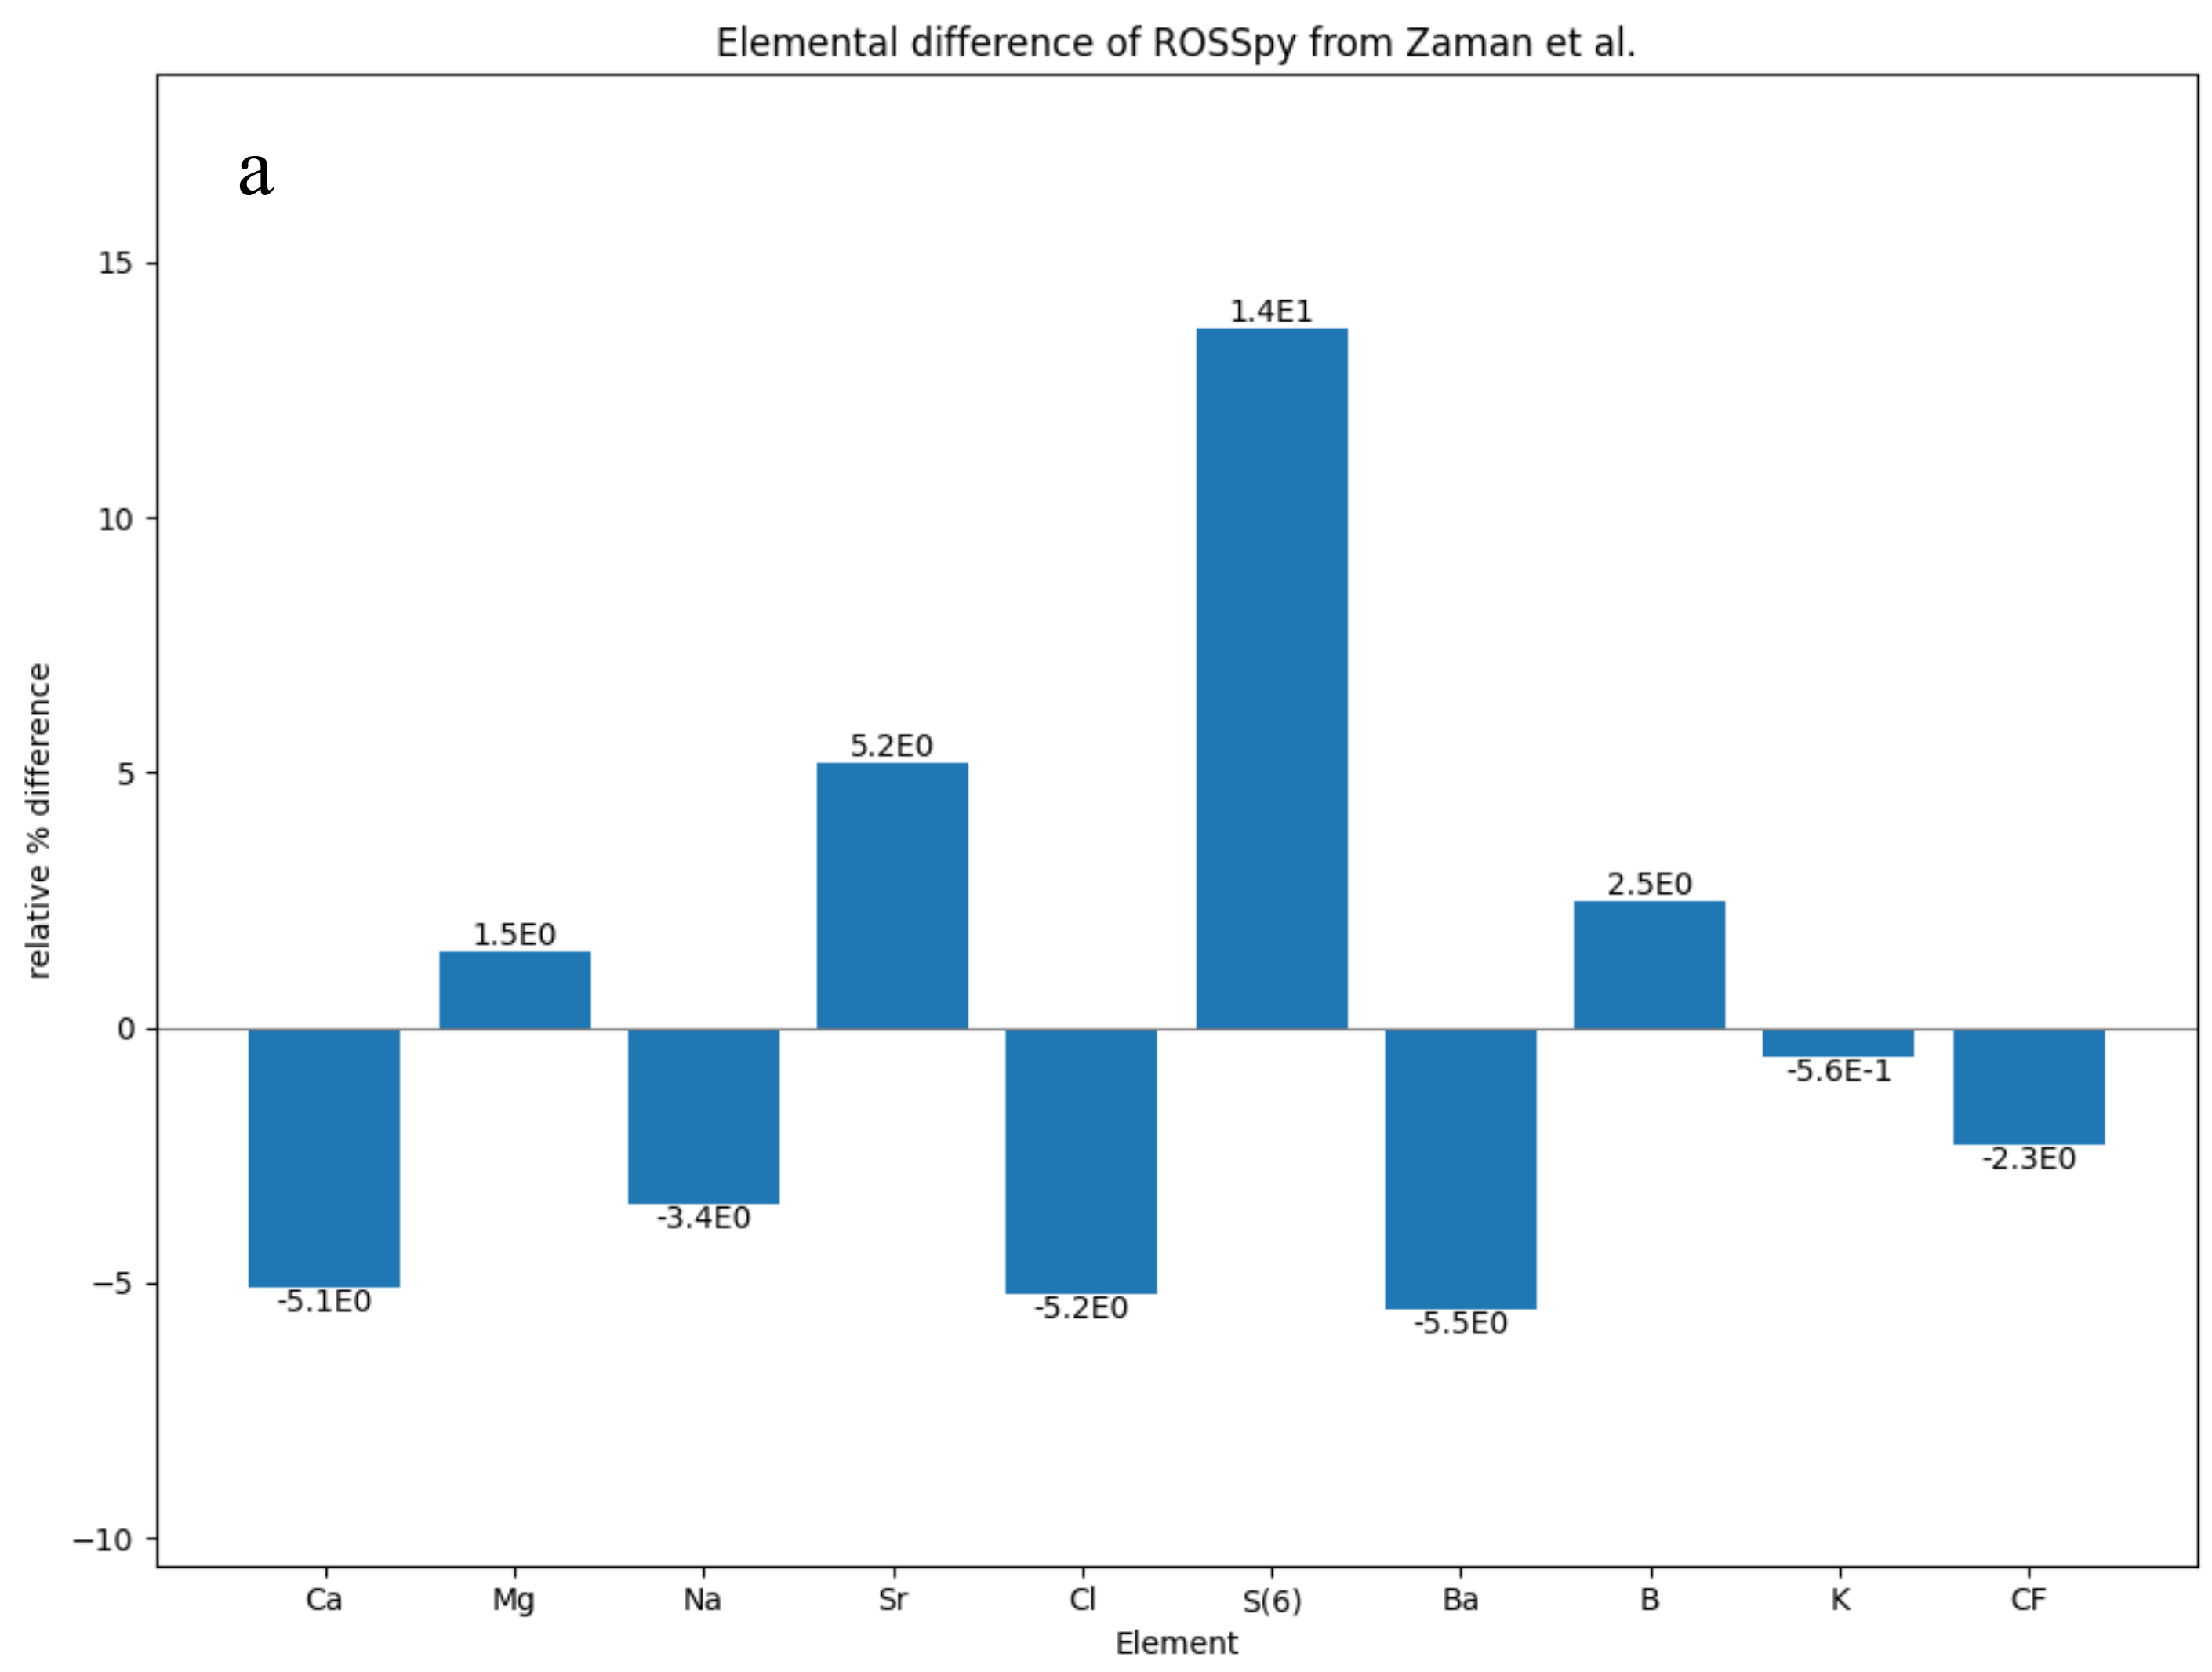
\includegraphics[width=\linewidth]{images/ROSSpy/case_studies/Zaman_comparison.png}} \\ \midrule
        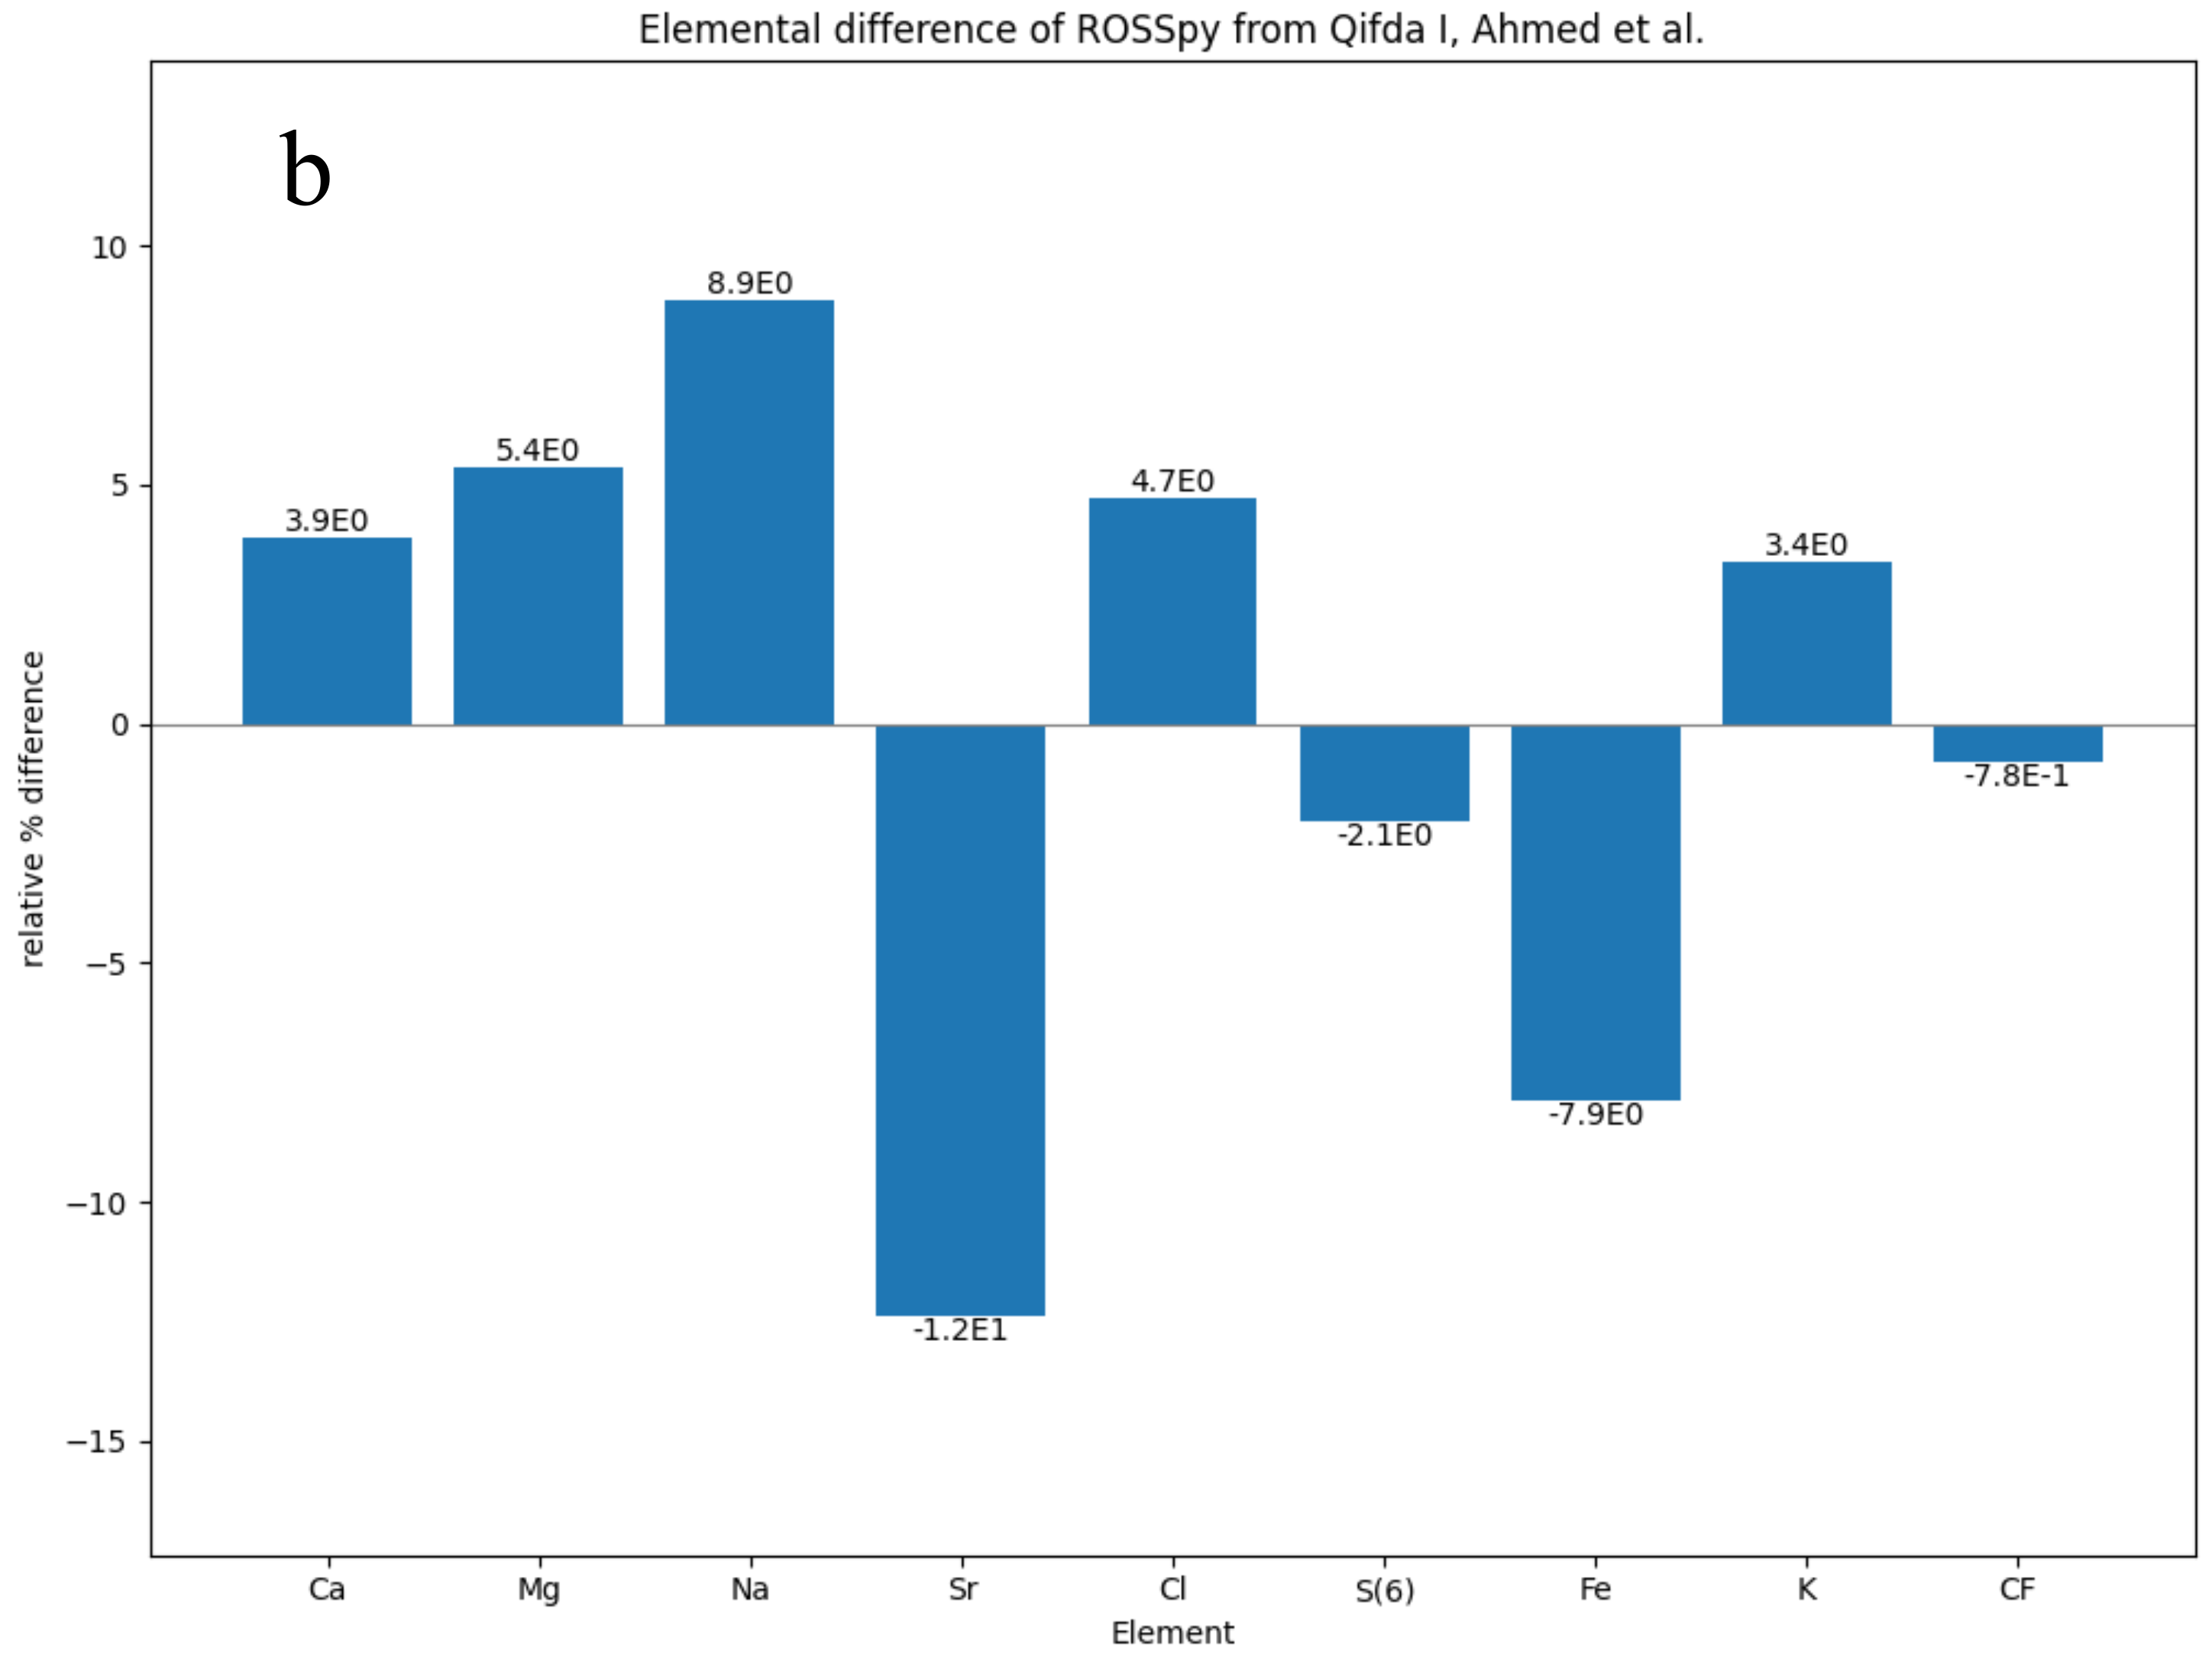
\includegraphics[width=0.49\linewidth]{images/ROSSpy/case_studies/Ahmed_comparison.png} & 
        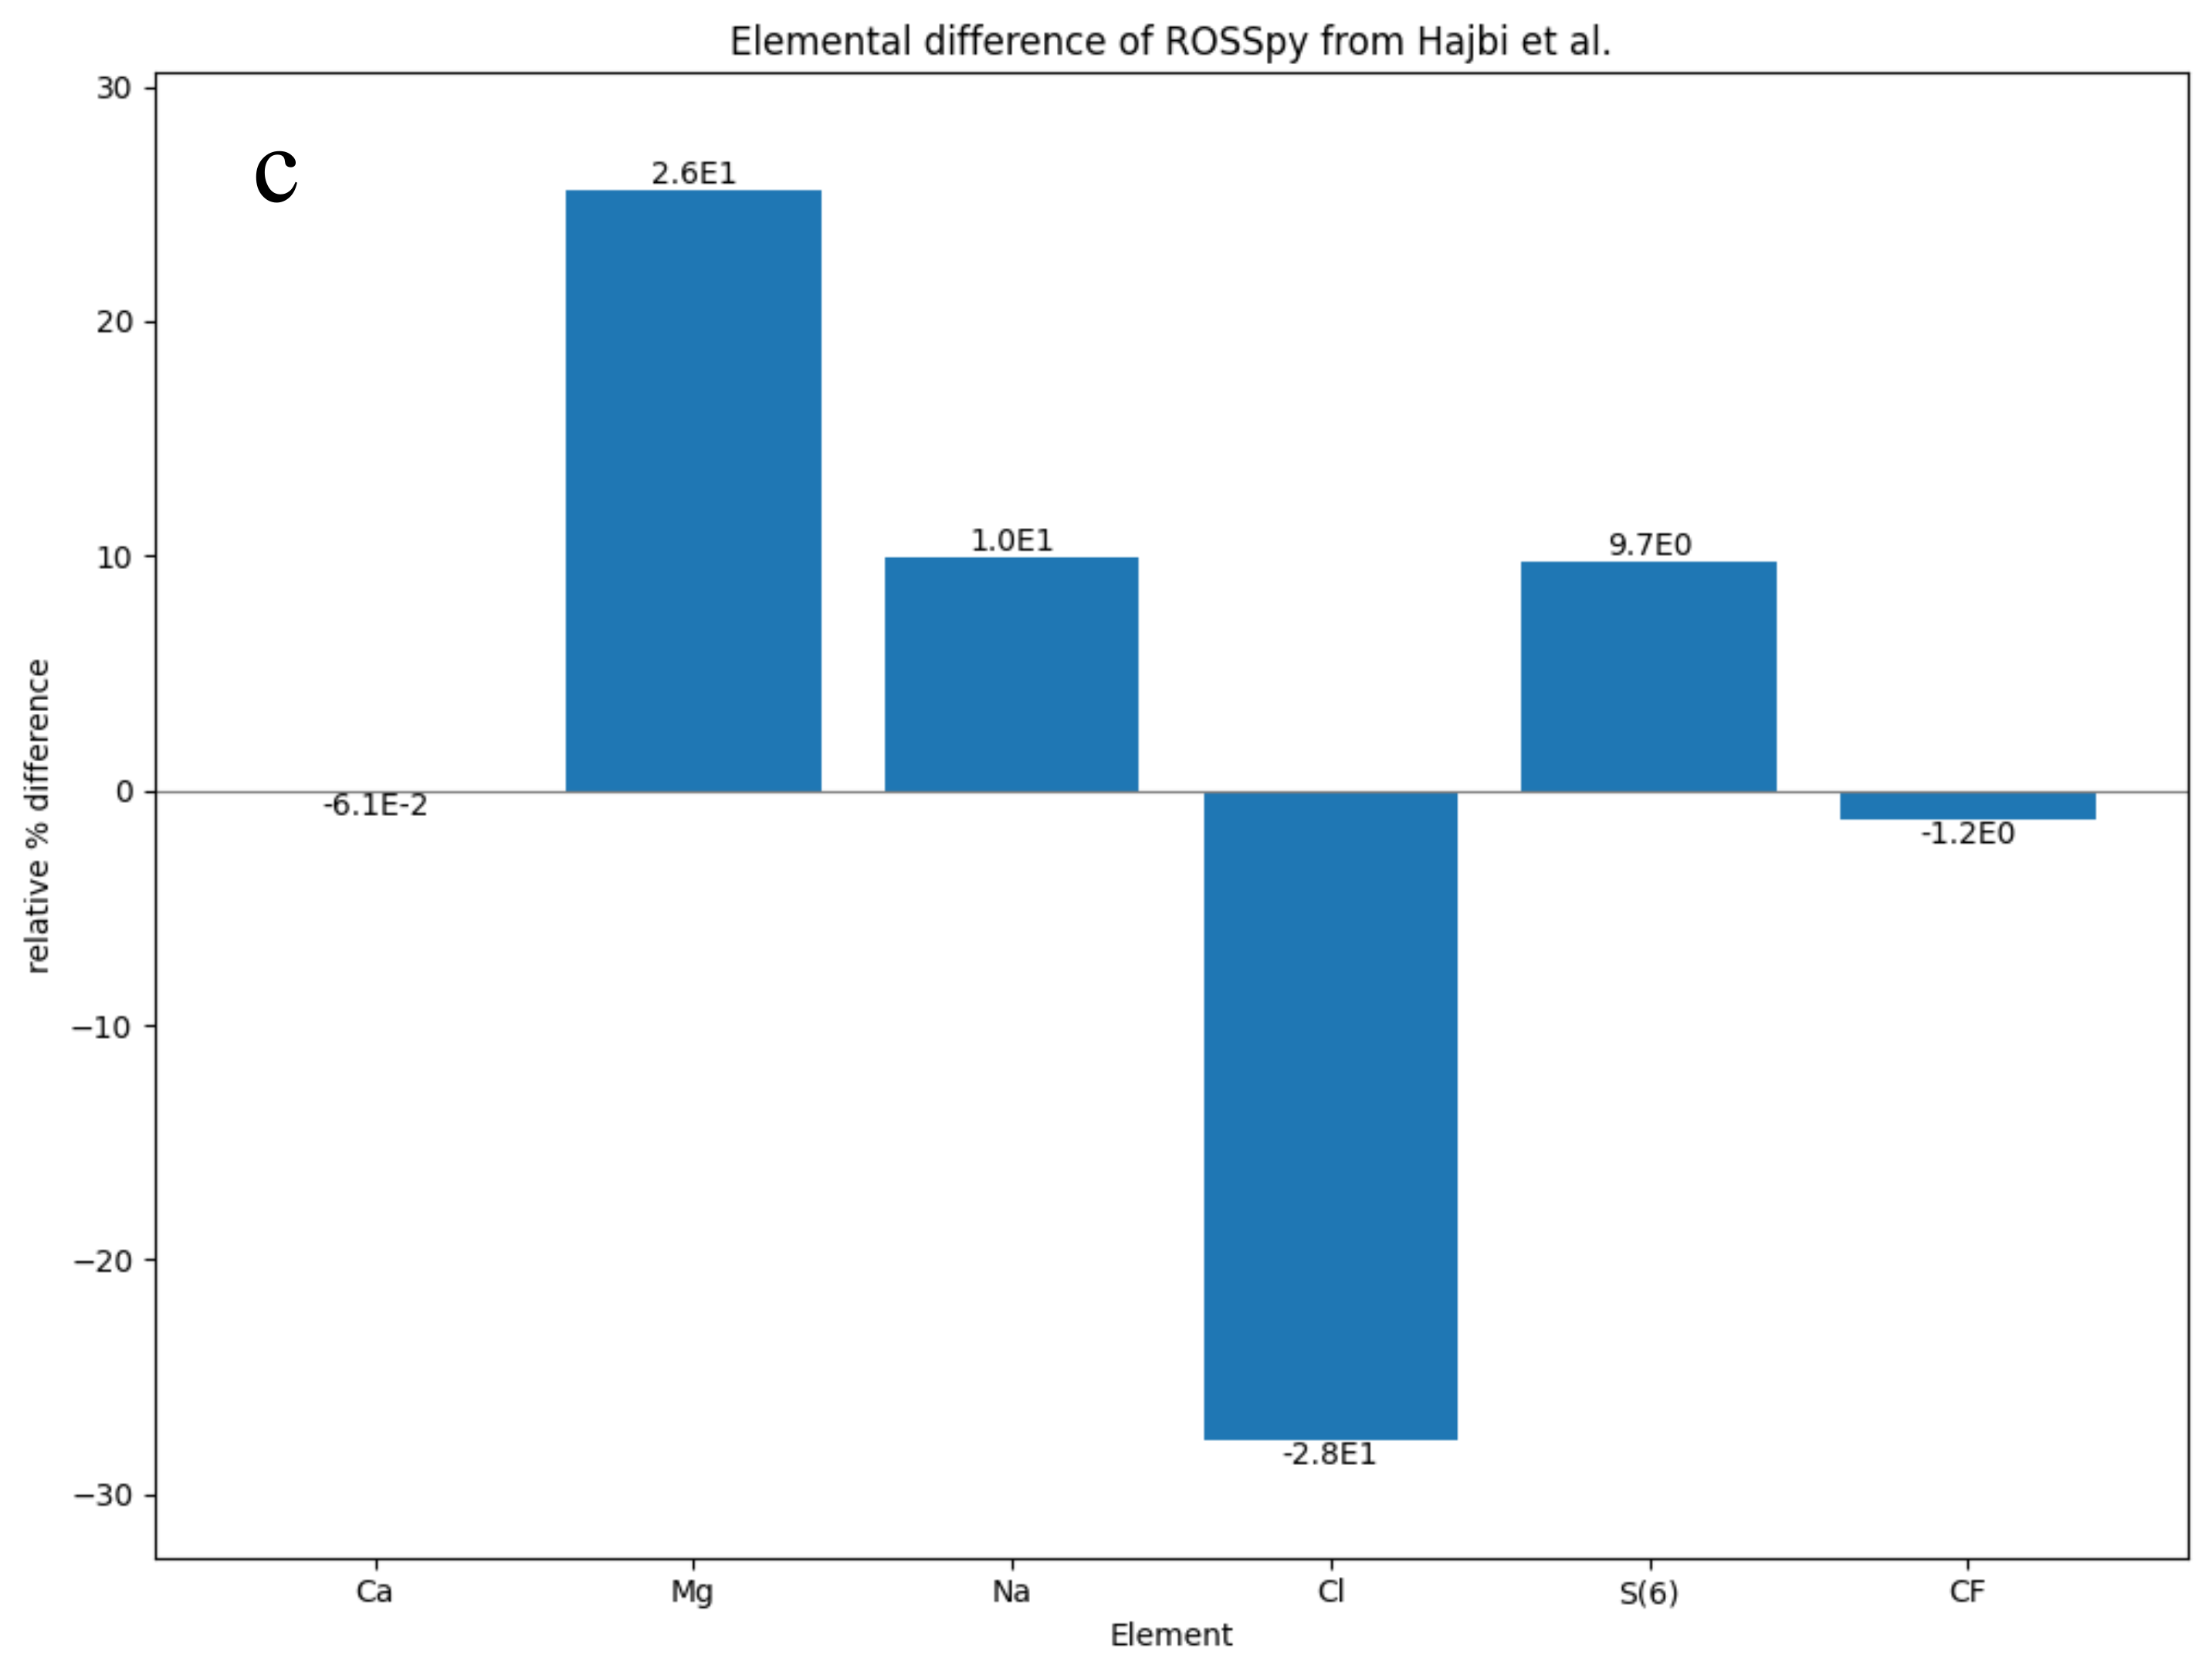
\includegraphics[width=0.49\linewidth]{images/ROSSpy/case_studies/Hajbi_comparison.png} \\ \bottomrule
    \end{tabular}
    \caption{
        The \%-error between predicted and experimental brine concentrations from RO plants. Panels a-c) correspond to comparisons with the Zaman et al. \cite{Zaman2015DownstreamCompounds}, Ahmed et al. \cite{Ahmed2001BrineEmirates}, and Hajbi et al. \cite{Hajbi2010ReuseBrine} studies, respectively, and each possess different y-axis scales to best resolve the bars in each graph. The trend is that prediction accuracy is proportional to the quantity of parameterized ions. 
    }
    \label{bar_graphs}
\end{figure}


\subsection{Scaling}
The scaling predictions were verified qualitatively from experimental literature and quantitatively from theoretical calculations, since experimental literature that quantified scalants with feed geochemistry was not discovered.

\subsubsection{Quantitative}
The quantitative verification consisted of two simple cases of Gypsum precipitation. 1) The first case in Table \ref{gypsum_ice_table} consists of a solution with only $Ca^{2+}$ and $SO_4^{2-}$, where the ionic concentrations decreased by $0.01859$ moles while $0.01961$ moles of Gypsum precipitated. This 5\% discrepancy in mass balance is attributed to the printed PHREEQC values in this calculation neglecting diffusion within the feed solution, yet diffusion is considered in the final output of PHREEQC. 2) The second case in Table S1 evaluates Gypsum precipitation from desalinating the solution from the first case with that from the Red Sea, which only precipitates Gypsum in our model. The simple solution precipitated $0.181$ moles of Gypsum, while the Red Sea precipitated $0.194$ moles. This $+7\%$-error is attributed to ionic interactions within the Red Sea feed that are not present by the simple solution of only $Ca^{2+}$ and $SO_4^{2-}$. These subtle $[5,7]\%$ deviations, even without considering the coarse assumptions in these simple examples, are relatively minor in the context of other sources of error, such as feed measurements, and still elicit quantitative consistency in scaling predictions.

\begin{table}
    \centering
    \begin{tabular}{c|ccccc}
      \toprule
       & $Ca^{2+}$ & $+$ & $SO_4^{2-}$ & $\leftrightharpoons$ & $CaSO_4$ \\
      \midrule
      I & $0.3545$ && $1.816$ && $0$ \\
      C & $-0.01859$ && $-0.01859$ && $+0.01961$ \\
      F & $0.3360$ && $1.797$ && $0.01961$ \\
      \bottomrule
    \end{tabular}
    \caption{
        Gypsum precipitation according to the ICE (Initial, Change, Equilibrium) framework, except that "Equilibrium" (E) is replaced with "Final" (F) since the system does not completely reach equilibrium within the RO module. The $5\%-error$ in row C, between the changes in ionic and Gypsum moles, suggests a subtle discrepancy in mass balance of PHREEQC; however, this is attributed to PHREEQC printing values before diffusion is incorporated in the calculations, per David Parkhurst. 
      }
    \label{gypsum_ice_table}
\end{table}

\subsubsection{Qualitative}
The scaling predictions were qualitatively verified through three experimental studies. 

\paragraph{Karabelas et al., 2020 \cite{Karabelas2020ScalingTools}}
This study inspired features of ROSSpy by reviewing the state-of-the-art, and future directions, for predictive scaling software. The study also, importantly, describes in its Supporting Information scalants that were observed after desalination with defined conditions. Scaling predictions from these conditions in Figure \ref{qualitative_scaling}a, over a few PHREEQC databases, match the reported scalants ("Calcite but not Gypsum" and a "few other salts, such as Barite and Dolomite, could also deposit at downstream...") in numerous aspects: 1) Calcite was the primary scalant; 2) Gypsum was not observed; 3) a few other salts precipitated, including Dolomite and Barite, depending upon the PHREEQC database; and 4) these other salts precipitated primarily in the downstream portion of the module.  

\paragraph{Karabelas et al., 2014 \cite{Karabelas2014IncipientChannels}}
This study elucidates the mechanisms of incipient scaling from RO desalination -- with Gypsum as the archetypal scalant \cite{Lyster2009CoupledModule}. The ID 28SC trial, which was the most thoroughly described trial, was simulated and Gypsum was the only predicted scalant in Figure \ref{qualitative_scaling}b, just as the reported scalant.  

\paragraph{Lee et al., 2009 \cite{Lee2009MembraneWastewater}}
This study evaluates the use of a membrane bioreactor -- a hollow-fiber membrane module design that is mechanistically similar to RO and thus can be represented by our model -- to treat wastewater. The wastewater filtration system was simulated, and the only predicted scalant was Calcite in Figure \ref{qualitative_scaling}c, just as the reported scalant.

\begin{figure}
    \begin{tabular}{c|c}
        \multicolumn{2}{c}{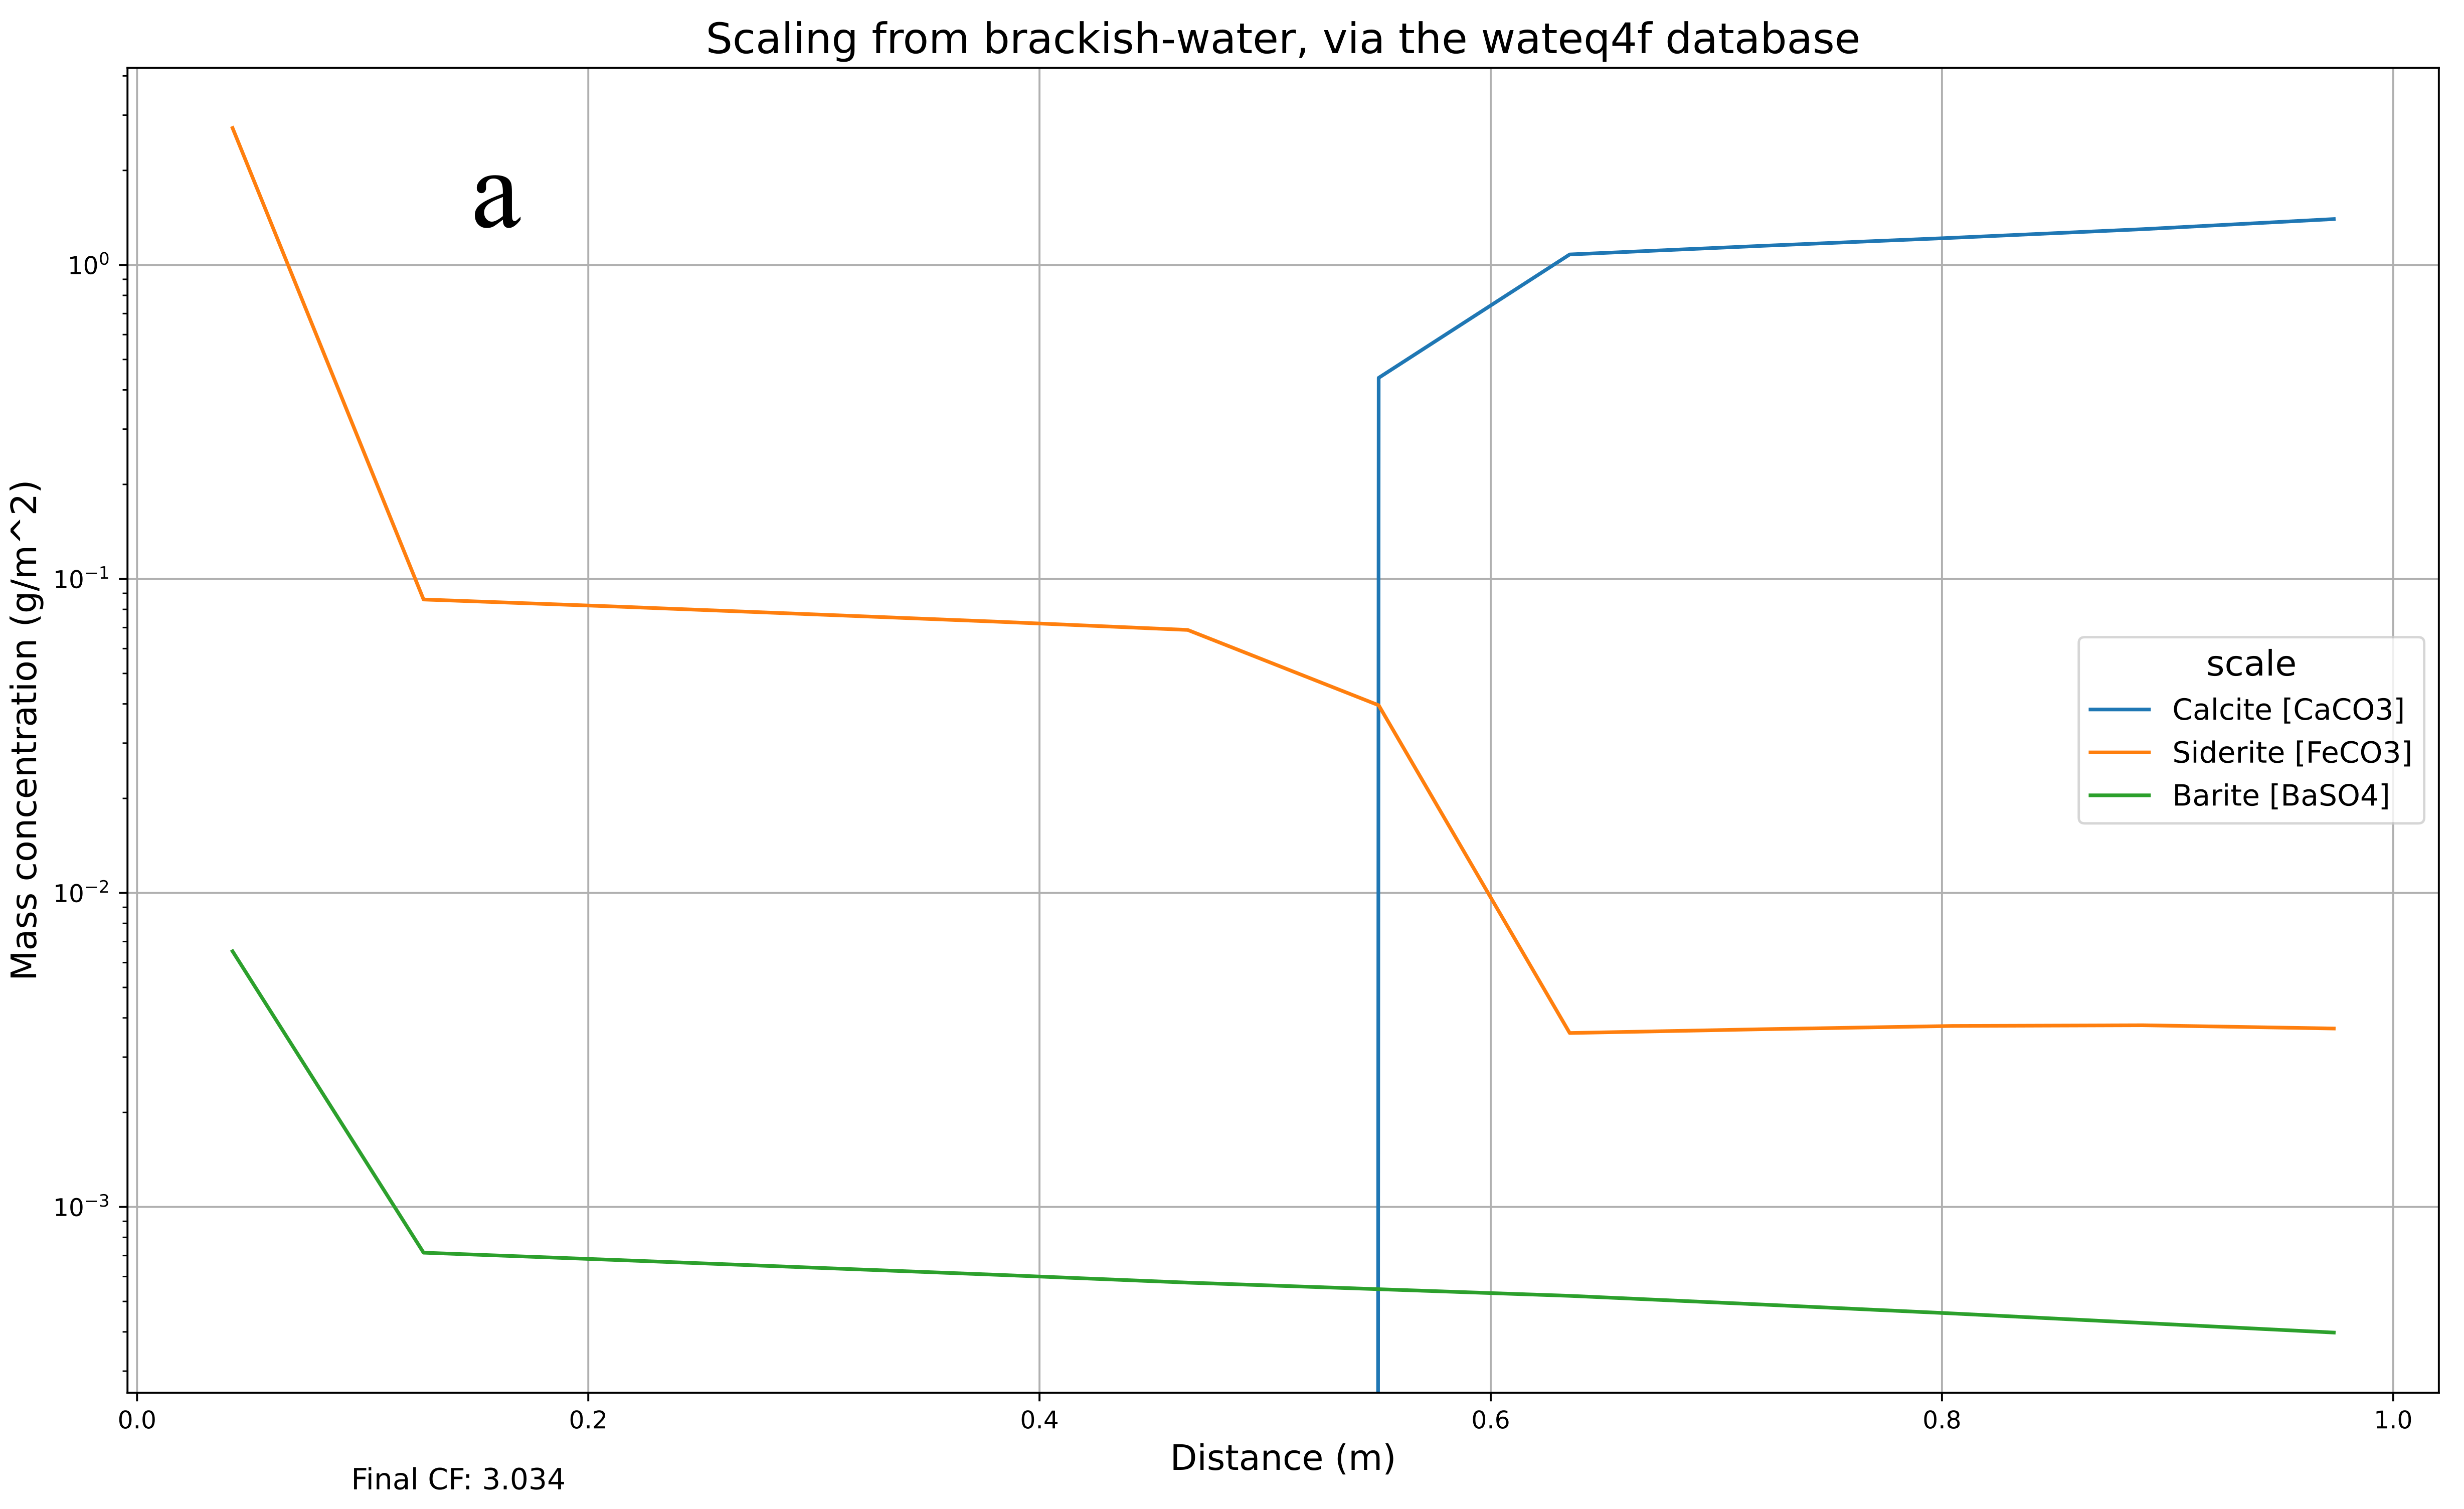
\includegraphics[width=\linewidth]{images/ROSSpy/case_studies/Karabelas_2020_wateq4f.png}} \\
        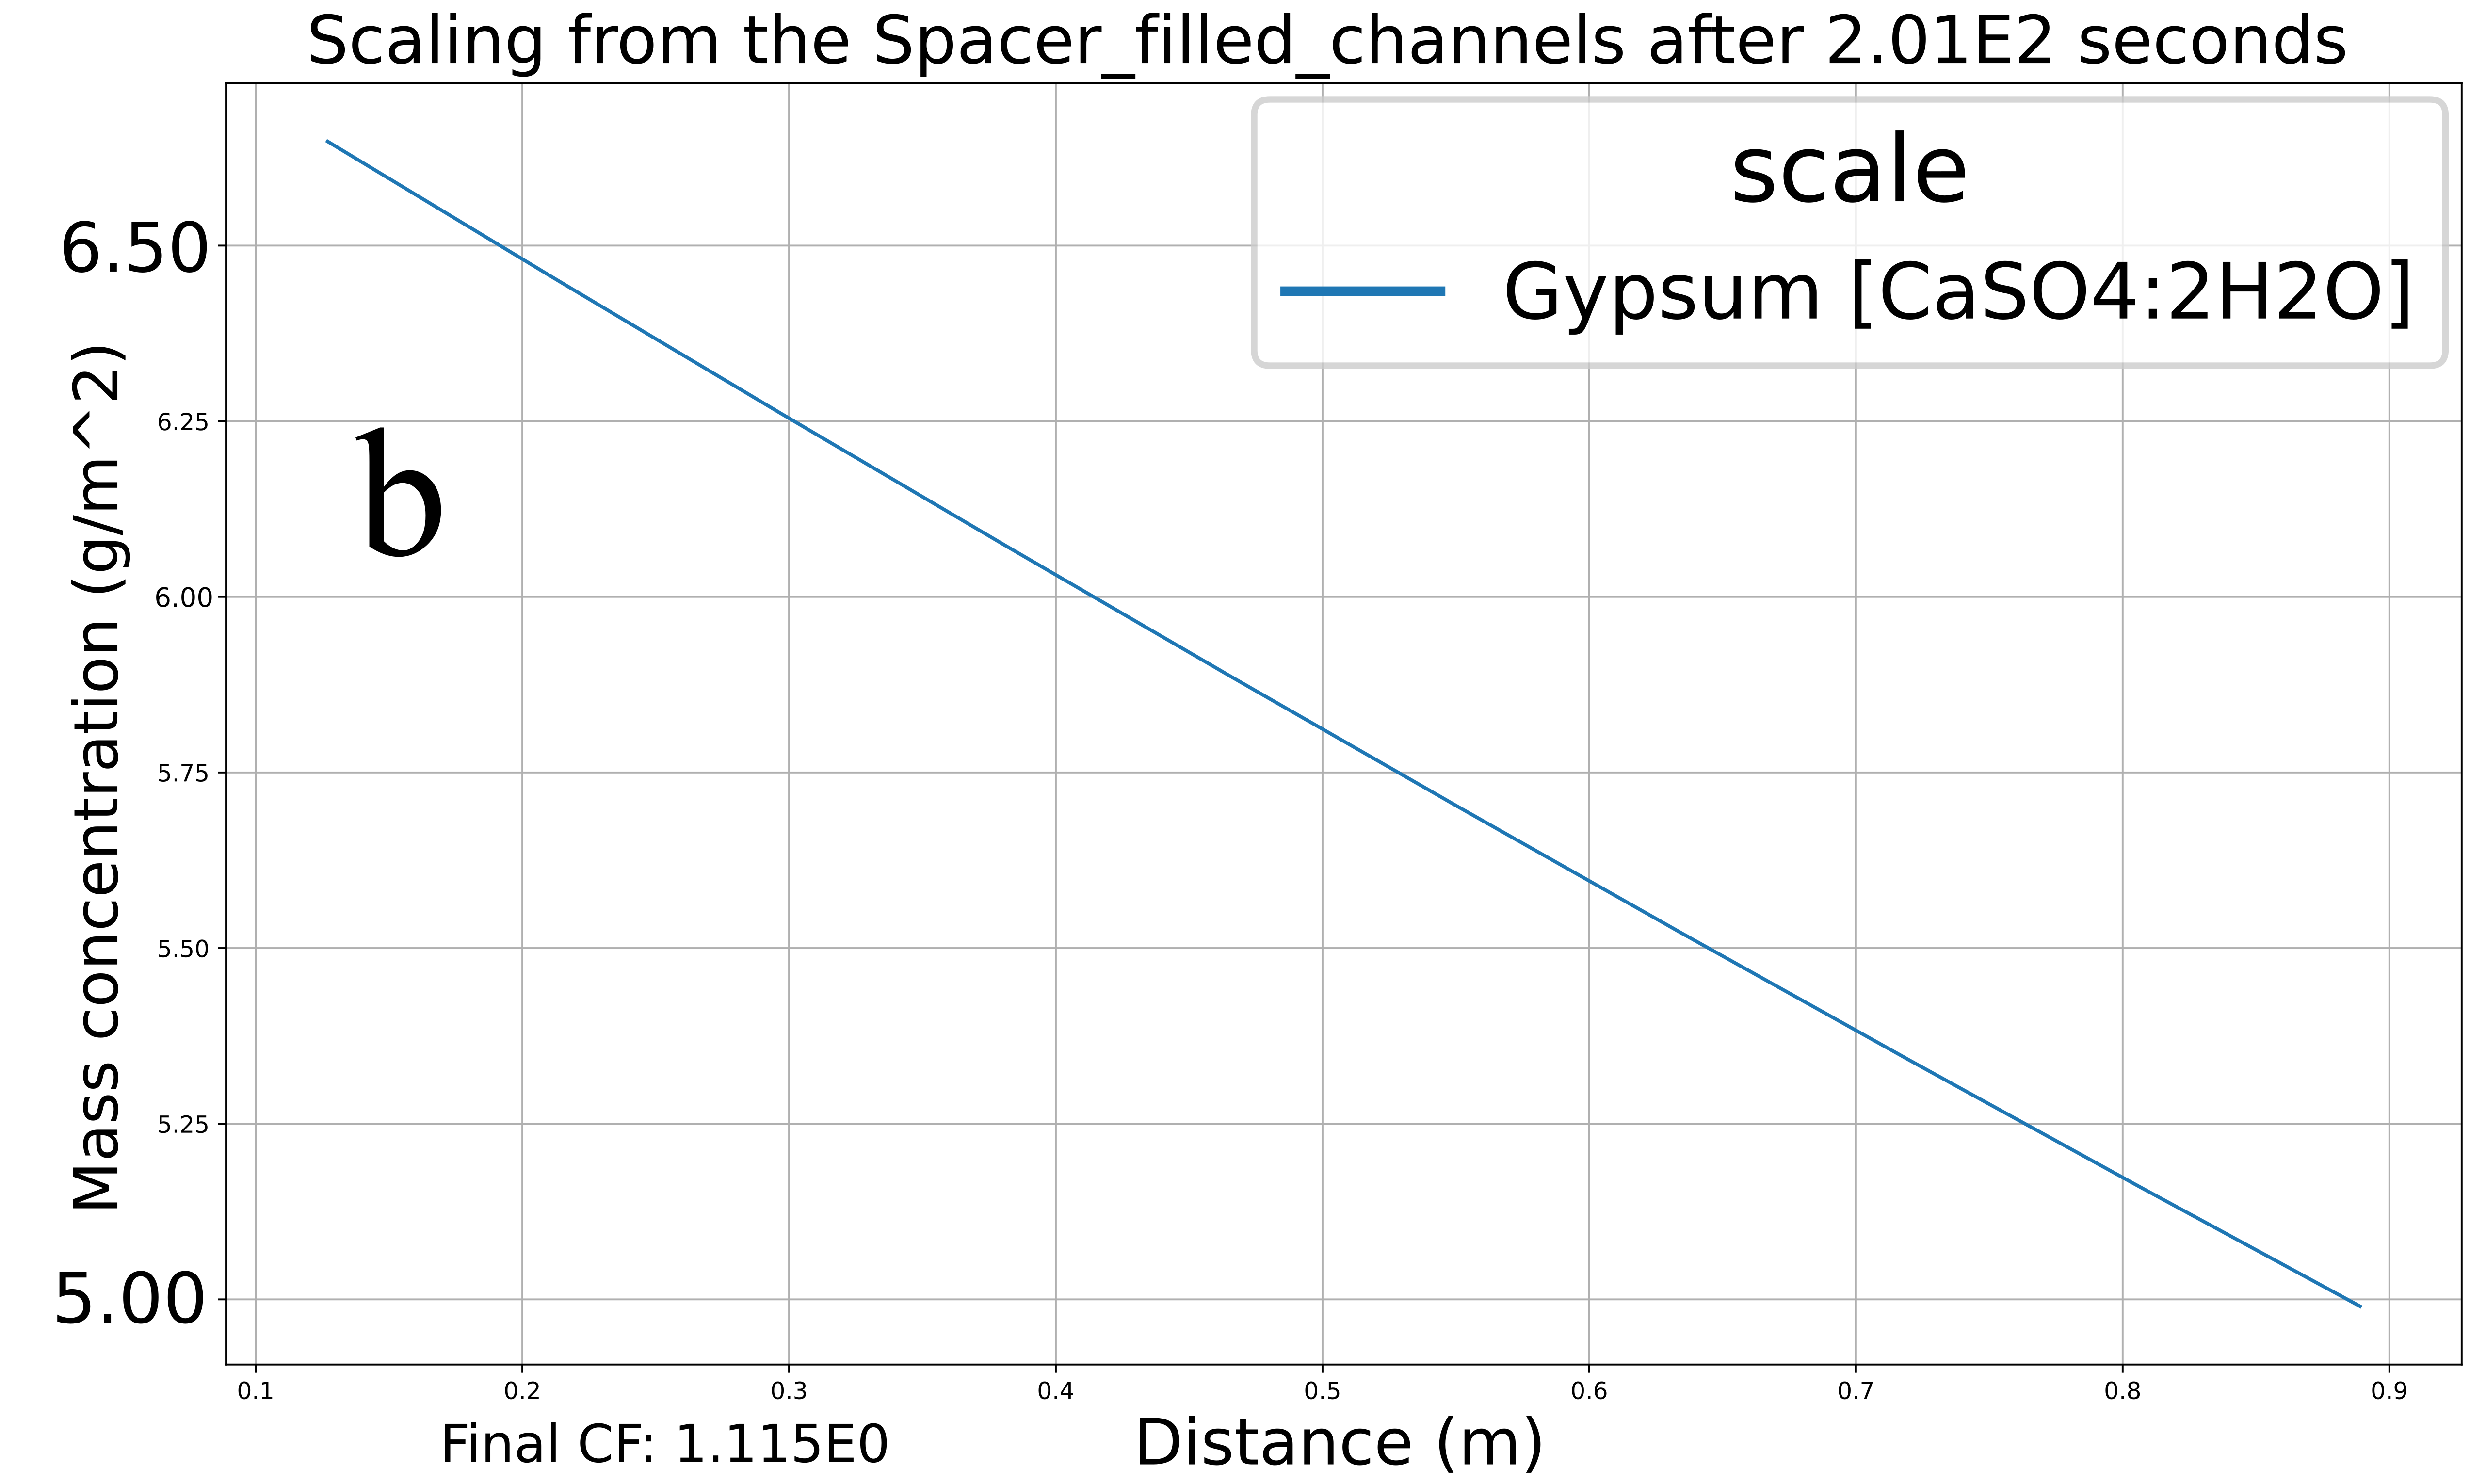
\includegraphics[width=0.49\linewidth]{images/ROSSpy/case_studies/Karabelas_2014_pitzer.png} 
        & 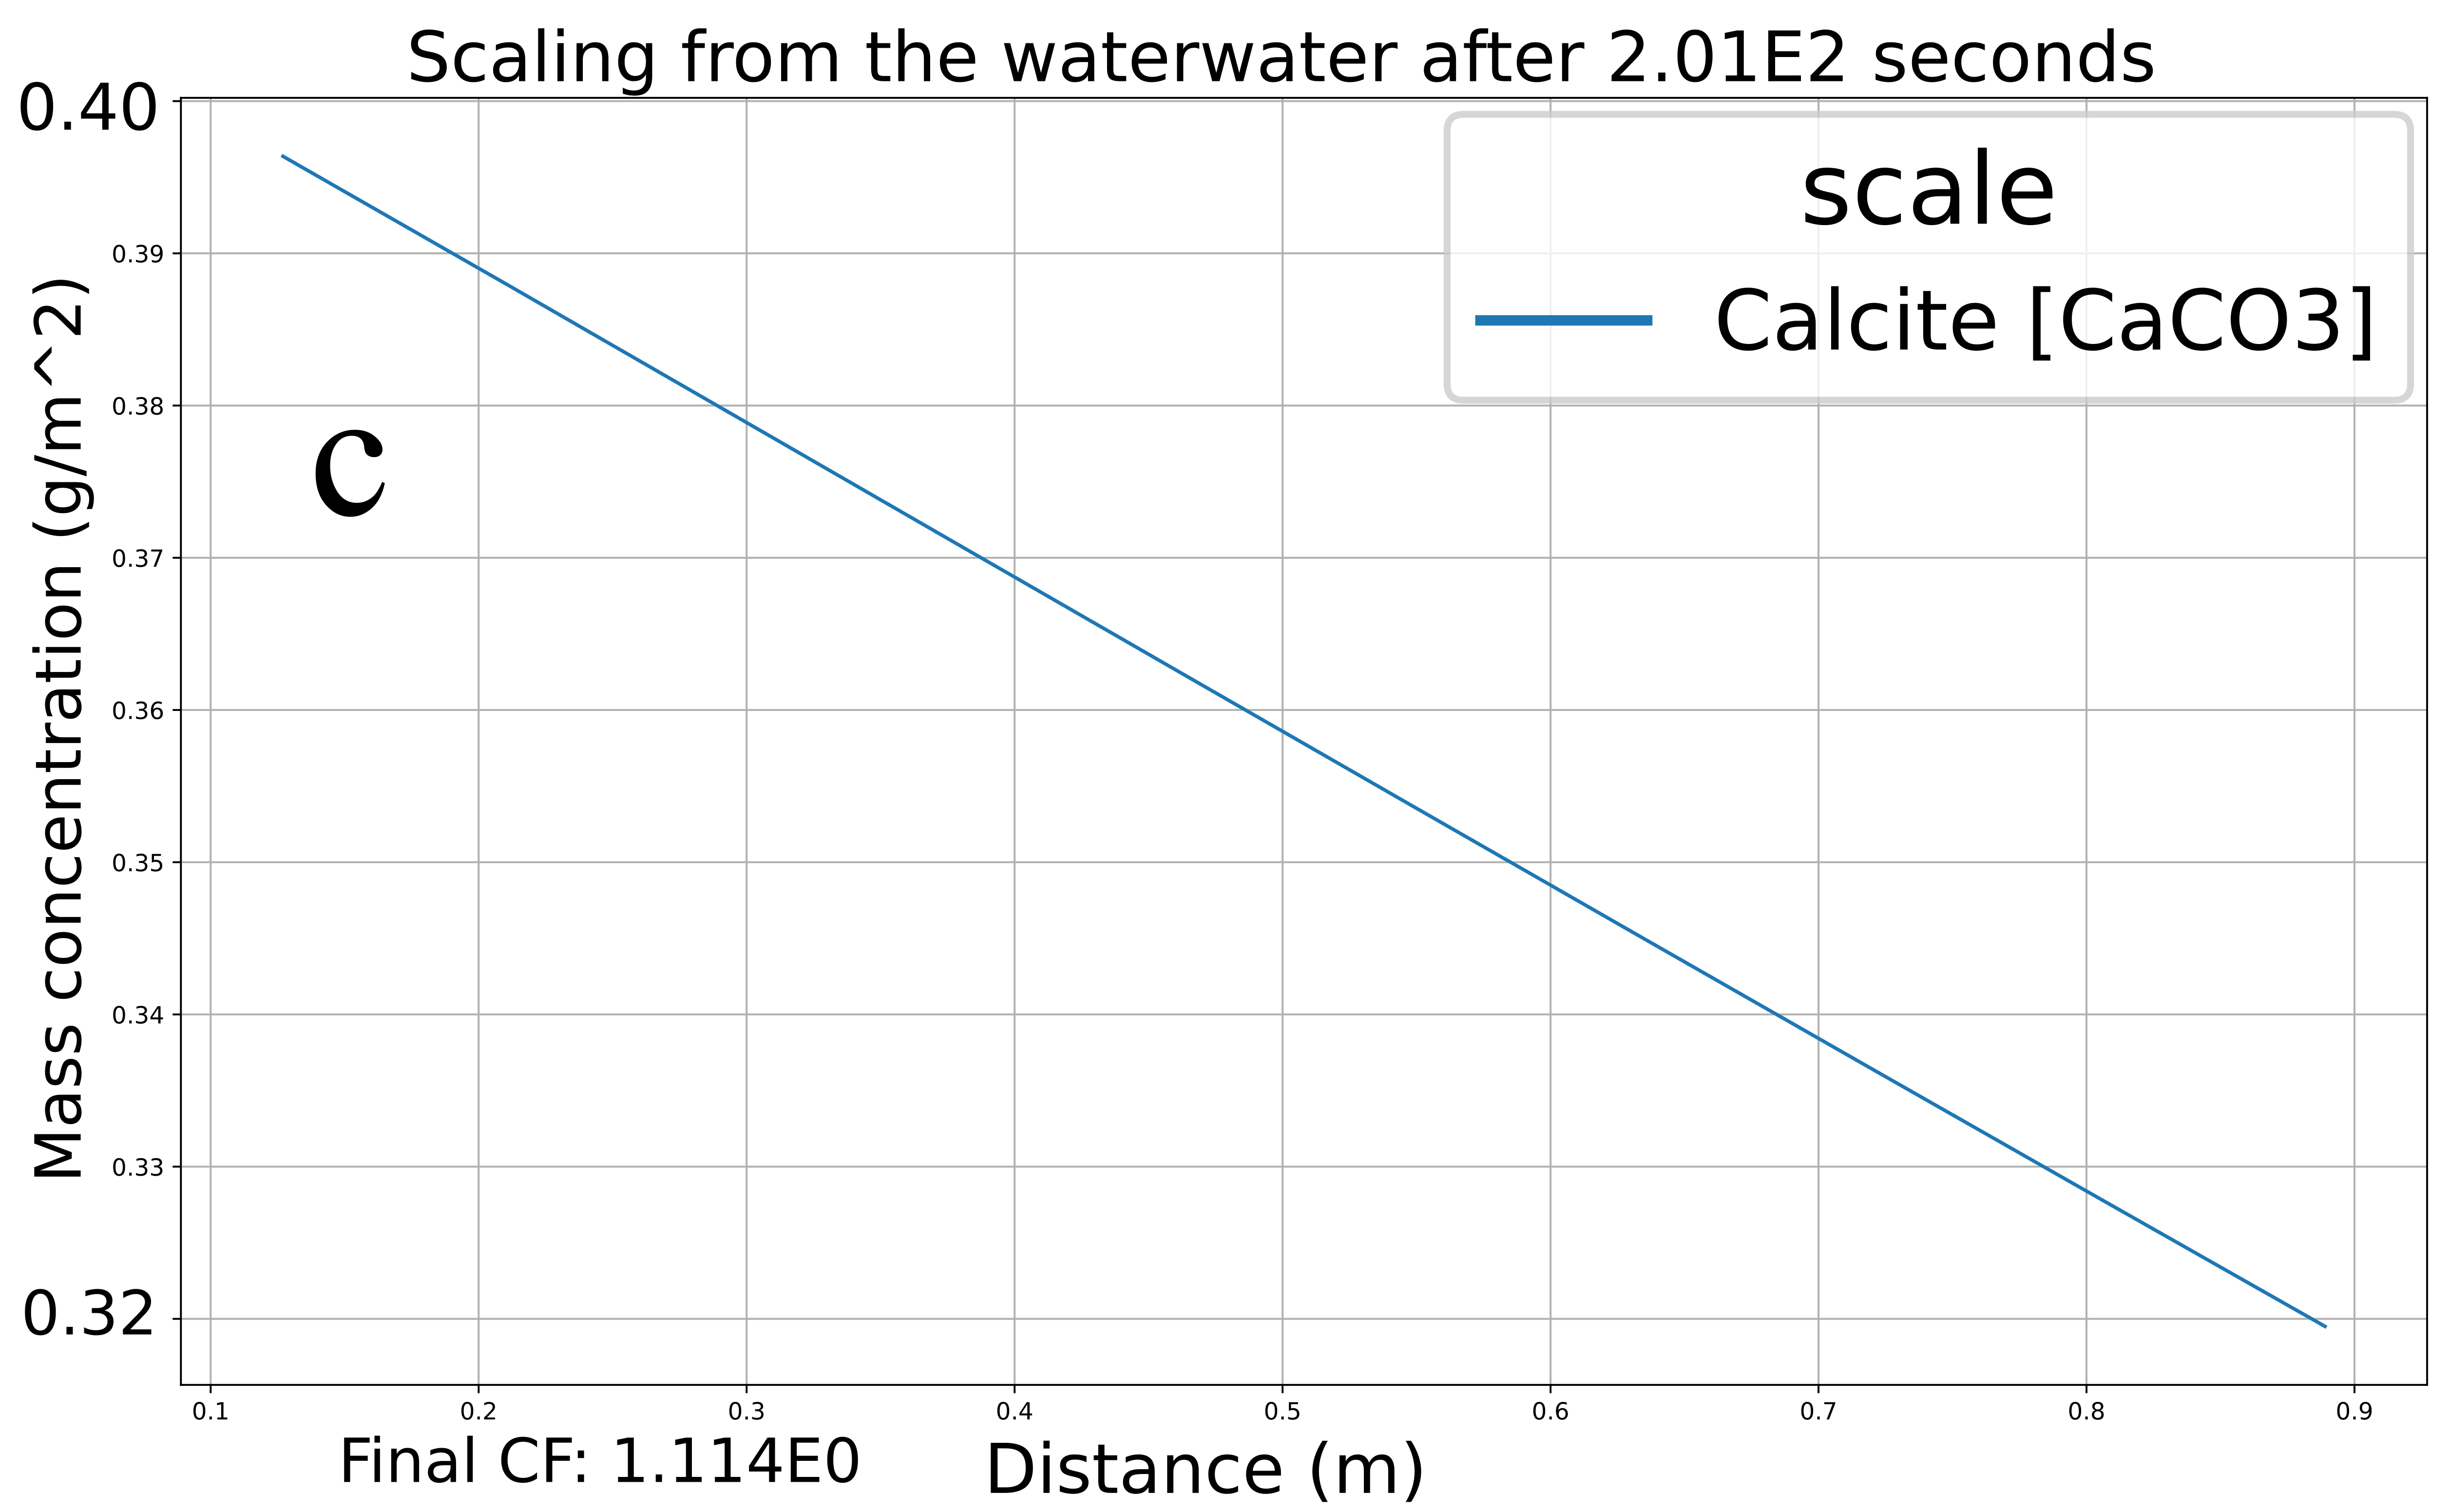
\includegraphics[width=0.49\linewidth]{images/ROSSpy/case_studies/Lee_pitzer.png} \\
    \end{tabular}
    \caption{
        The qualitative validation of scaling for a) multiple minerals from the Karabelas et al., 2020 study; b) Gypsum in the Karabelas et al., 2014 study; and c) Calcite in the Lee et al. study. 
    }
    \label{qualitative_scaling}
\end{figure}


\section{Sensitivity analyses}
A few sensitivity analyses were conducted with major variables in the following subsections. Additional sensitivity analyses of lesser parameters are presented in the Supporting Information.

\subsection{Database section}
The PHREEQC databases crucially 1) determines the set of minerals that can be simulated; 2) contains all of the kinetic, thermodynamic, and stoichiometric information of each mineral; and 3) employs a chemical activity model: e.g. Pitzer, Debye-H\"uckel, and Davies in Section 7 of the Supporting Information. The Pitzer model \cite{Pitzer1973ThermodynamicsEquations,Pitzer1974ThermodynamicsElectrolytes}, which is implemented in the pitzer PHREEQC database, is touted as being supremely accurate in the concentration range of desalination \cite{VandeLisdonk2001PredictionSystems,Sheikholeslami2004AssessmentUnits,Mohammad2007PredictionMembranes}; however, the narrow breadth of accepted ions and minerals may justify using other databases, such as wateq4, for complex or uncommon feed sources. Each of the 13 databases were simulated in desalinating the Red Sea, where the $Amm$, $Core10$, $LLNL$, and $Minteq.v4$ databases failed to numerically converge while the scaling predictions from the other $\frac{9}{13}$ databases are summarized in Figure \ref{database_selection}. The database selection evidently alters scaling predictions; thus, the database must be carefully selected for a given system after reviewing the PHREEQC User Manual or inquirying to the PHREEQC user forum \url{PHREEQCusers.org}.

\begin{figure}
    \centering
    \begin{tabular}{c|c}
        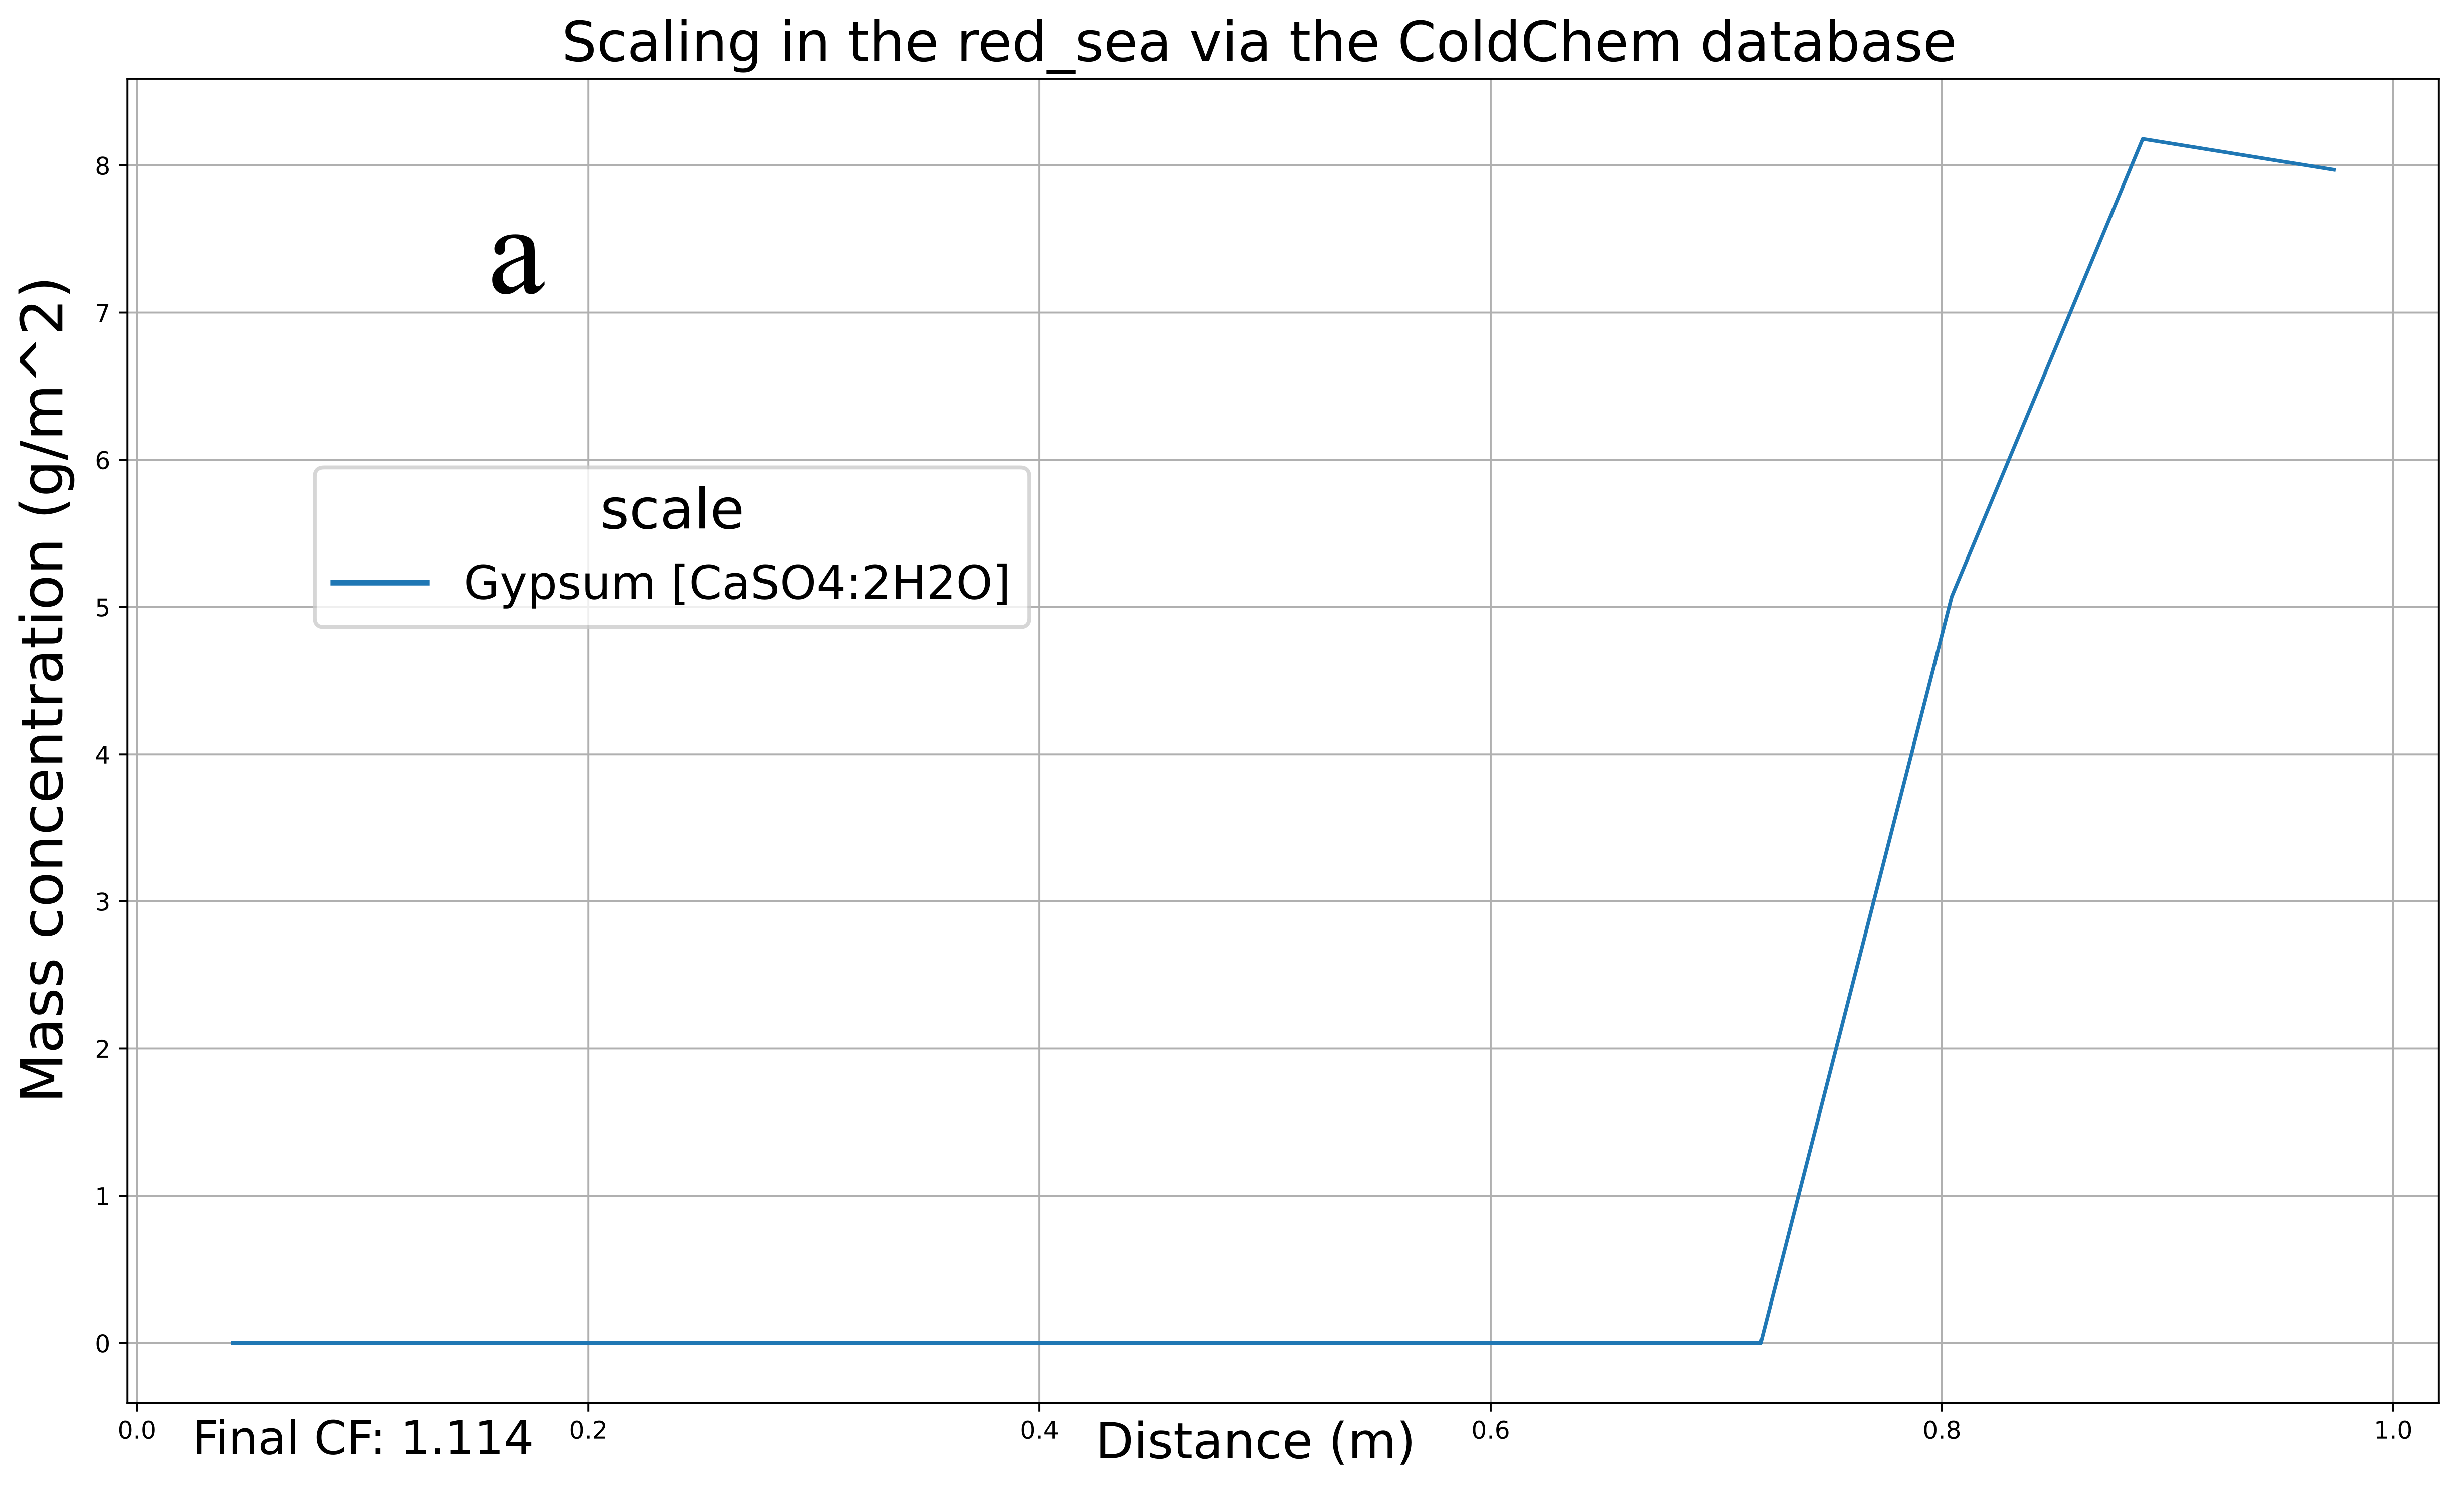
\includegraphics[width=0.49\textwidth]{images/ROSSpy/sensitivity_analyses/databases/ColdChem.png} 
        & 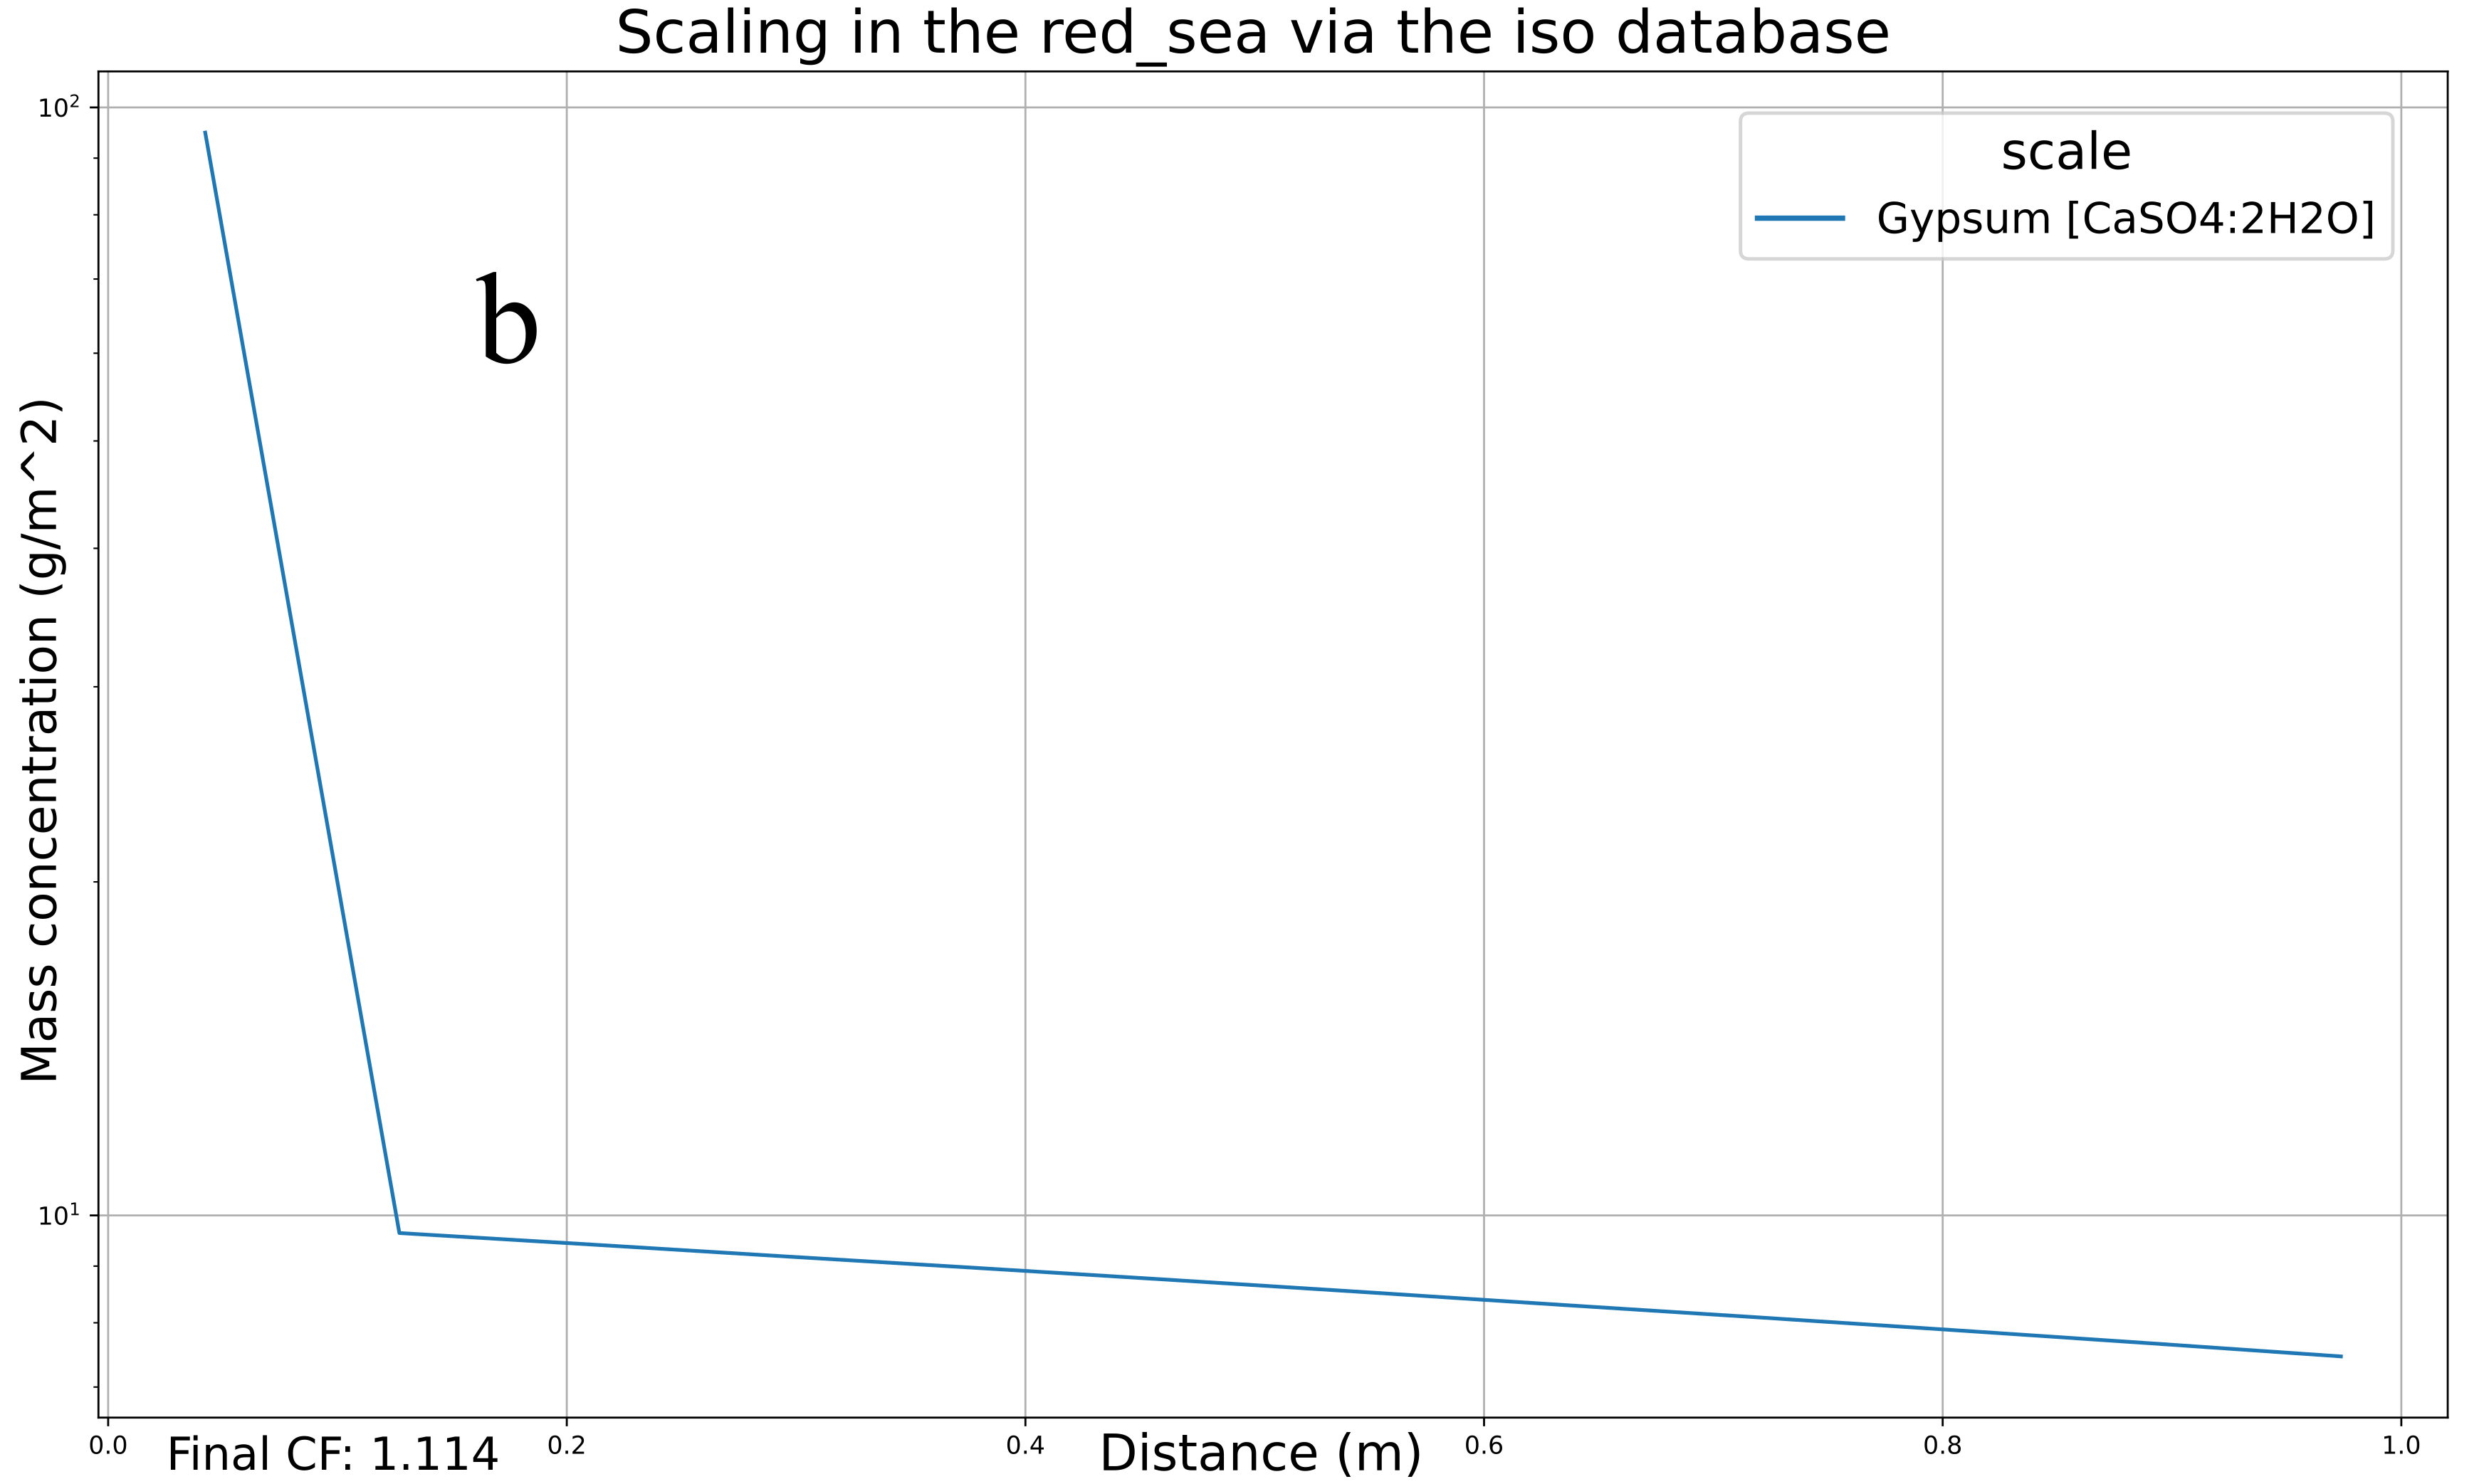
\includegraphics[width=0.49\textwidth]{images/ROSSpy/sensitivity_analyses/databases/Iso.png} \\ \midrule 
        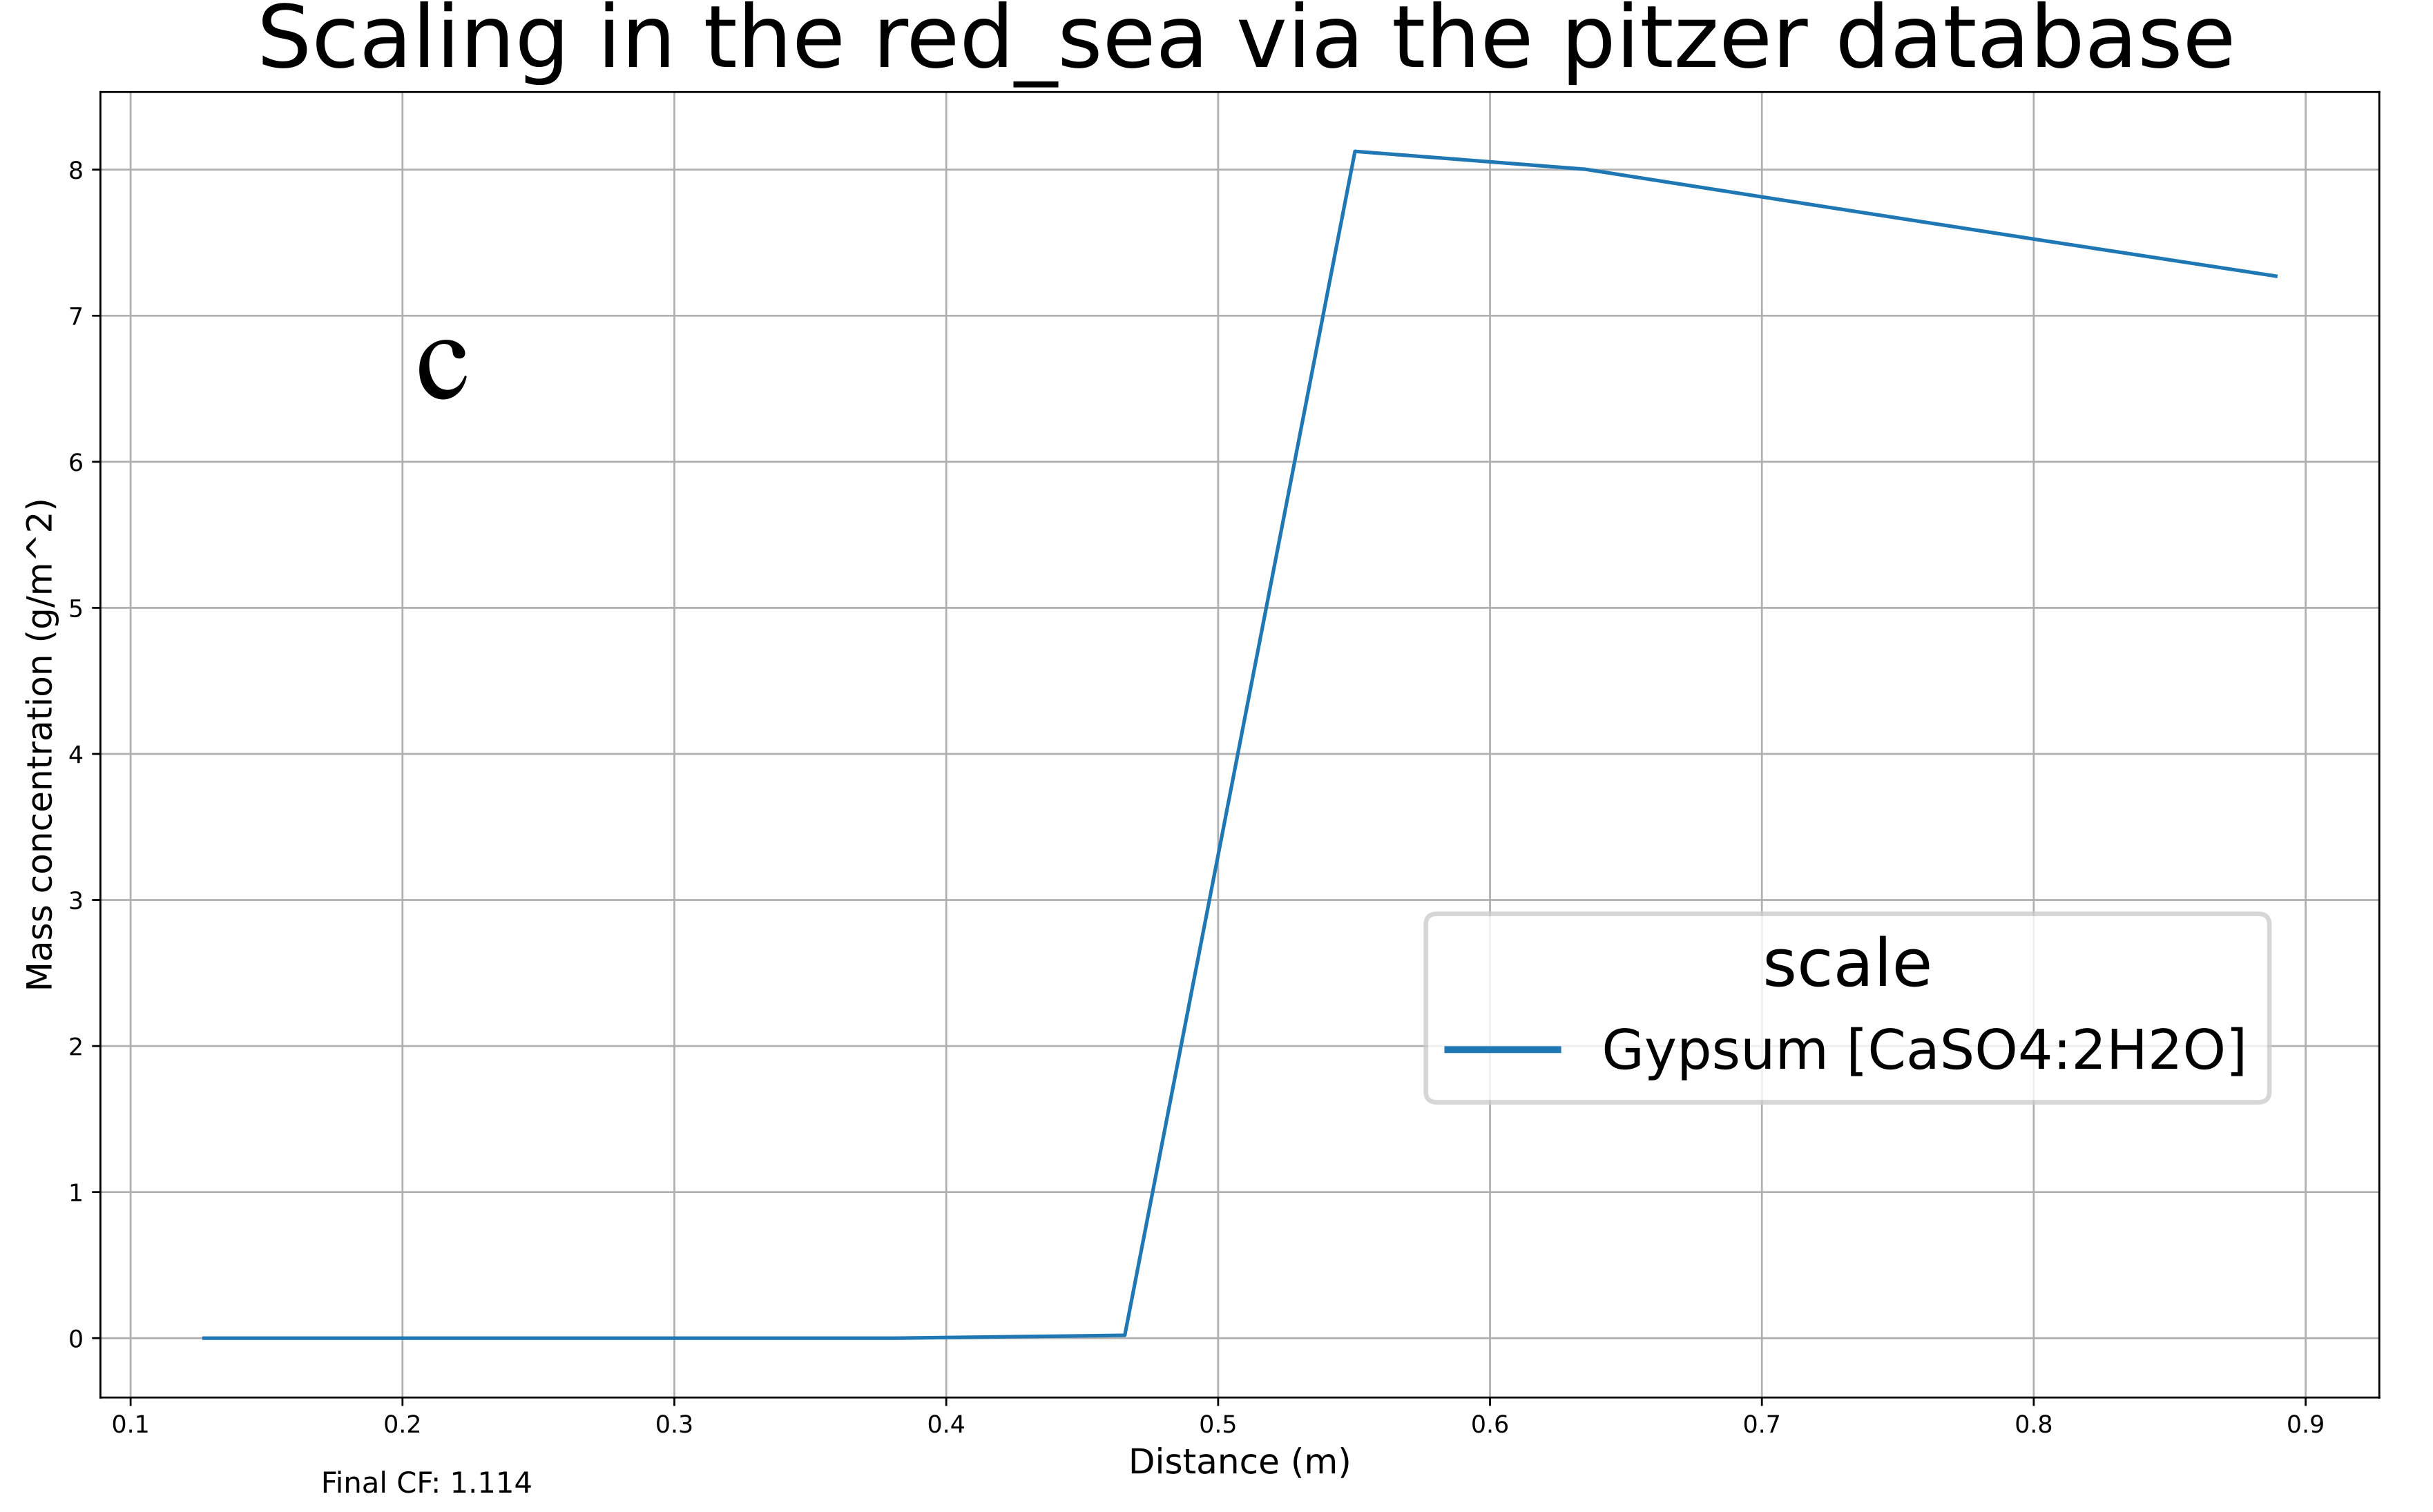
\includegraphics[width=0.49\textwidth]{images/ROSSpy/sensitivity_analyses/databases/Pitzer.png} 
        & 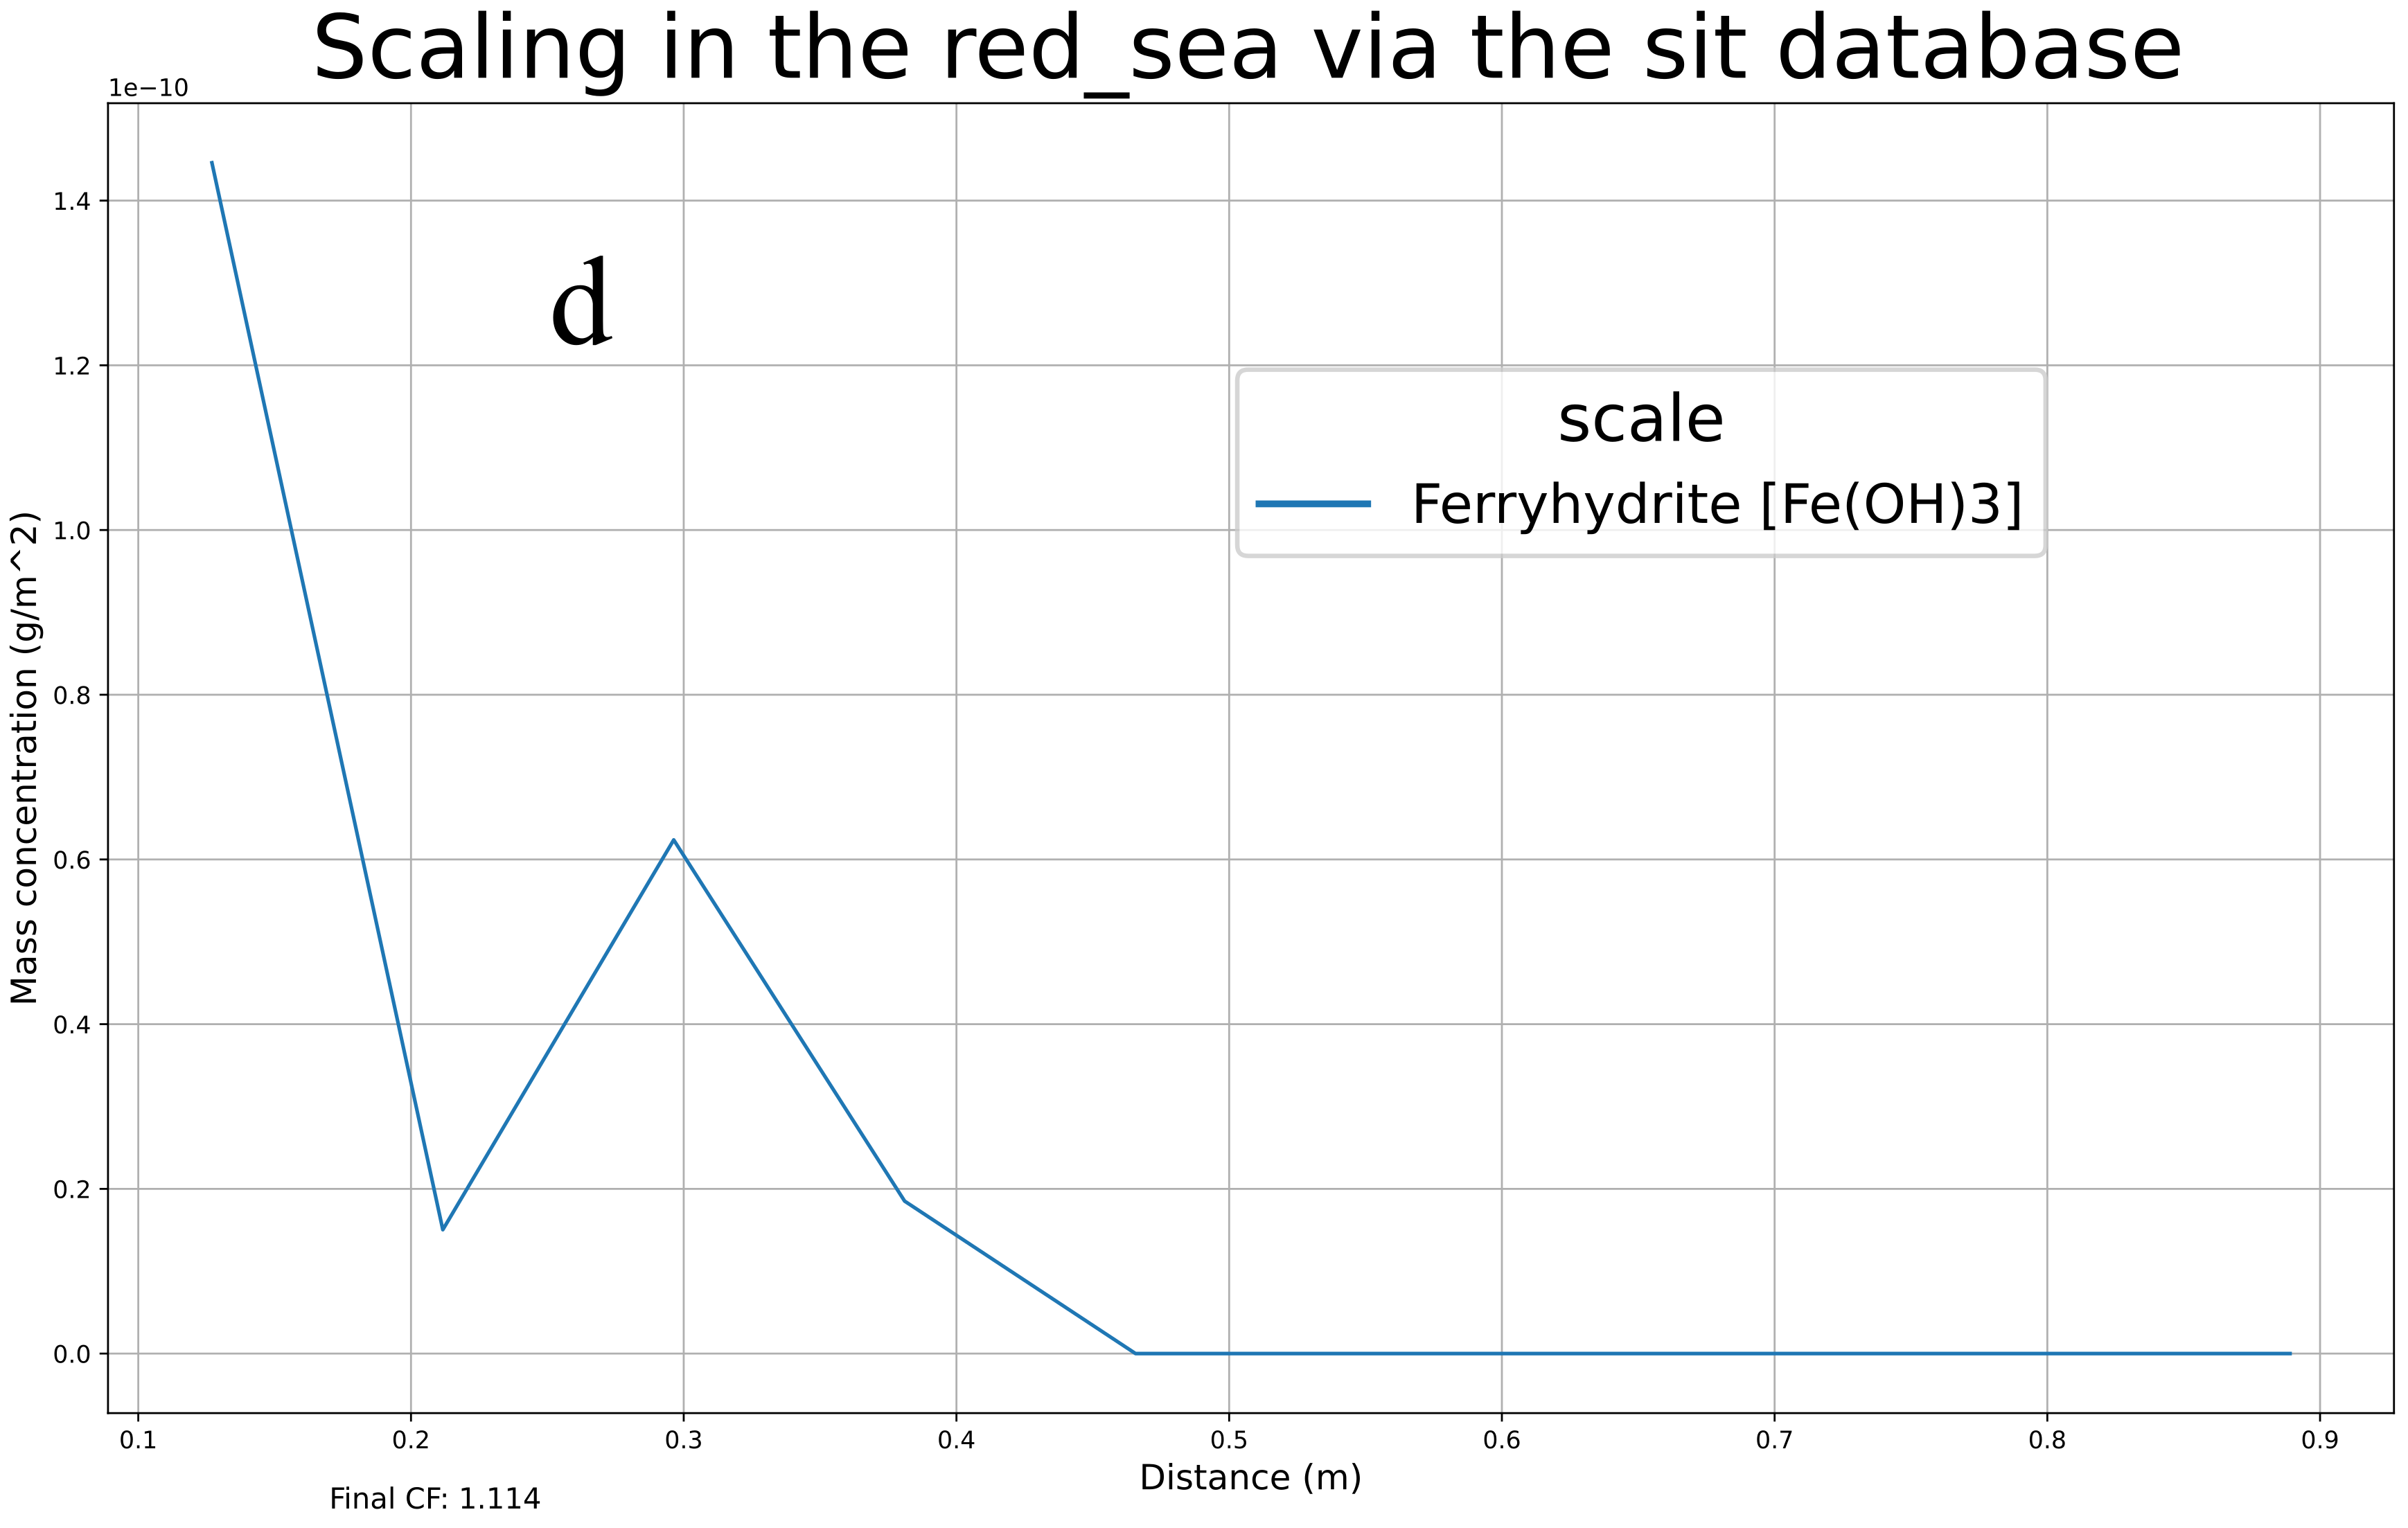
\includegraphics[width=0.49\textwidth]{images/ROSSpy/sensitivity_analyses/databases/Sit.png} 
        \\ \bottomrule
    \end{tabular}
    \caption{
        Scaling predictions from the a) ColdChem, b) Iso, c) Pitzer, and d) Sit databases, with otherwise identical simulation parameters. These subfigures represent the spectrum of similar yet distinct predictions of scaling during the database sensitivity analysis, and exemplify that the PHREEQC database should be deliberately selected after reviewing the PHREEQC documentation to discern which database is most appropriate for the feed geochemistry.
    }
    \label{database_selection}
\end{figure}

\subsection{Feed geochemistry}
The default feed waters were constructed from experimental geochemical literature into parameter files that are provided with ROSSpy. Users of ROSSpy are encouraged to simulate their own feed water while emulating the syntax of the default parameter files. We propose experimental data of numerous other water sources in Section 5 of the Supporting Information that can predicate feed water files; although, direct measurement of the simulated feed water is preferable to avoid significant influences of anthropogenic pollution \cite{Chen2008SourcesSea} and seasonality \cite{Sarthou2001SeasonalSea} in reported measurements. Thee default water sources, which include both natural seas and produced waters from oil wells, were contrasted in Figure \ref{feed_sources}, where the scaling and brine predictions differed significantly amongst these feed water sources. 

\begin{figure}
    \centering
    \begin{tabular}{c|c}
        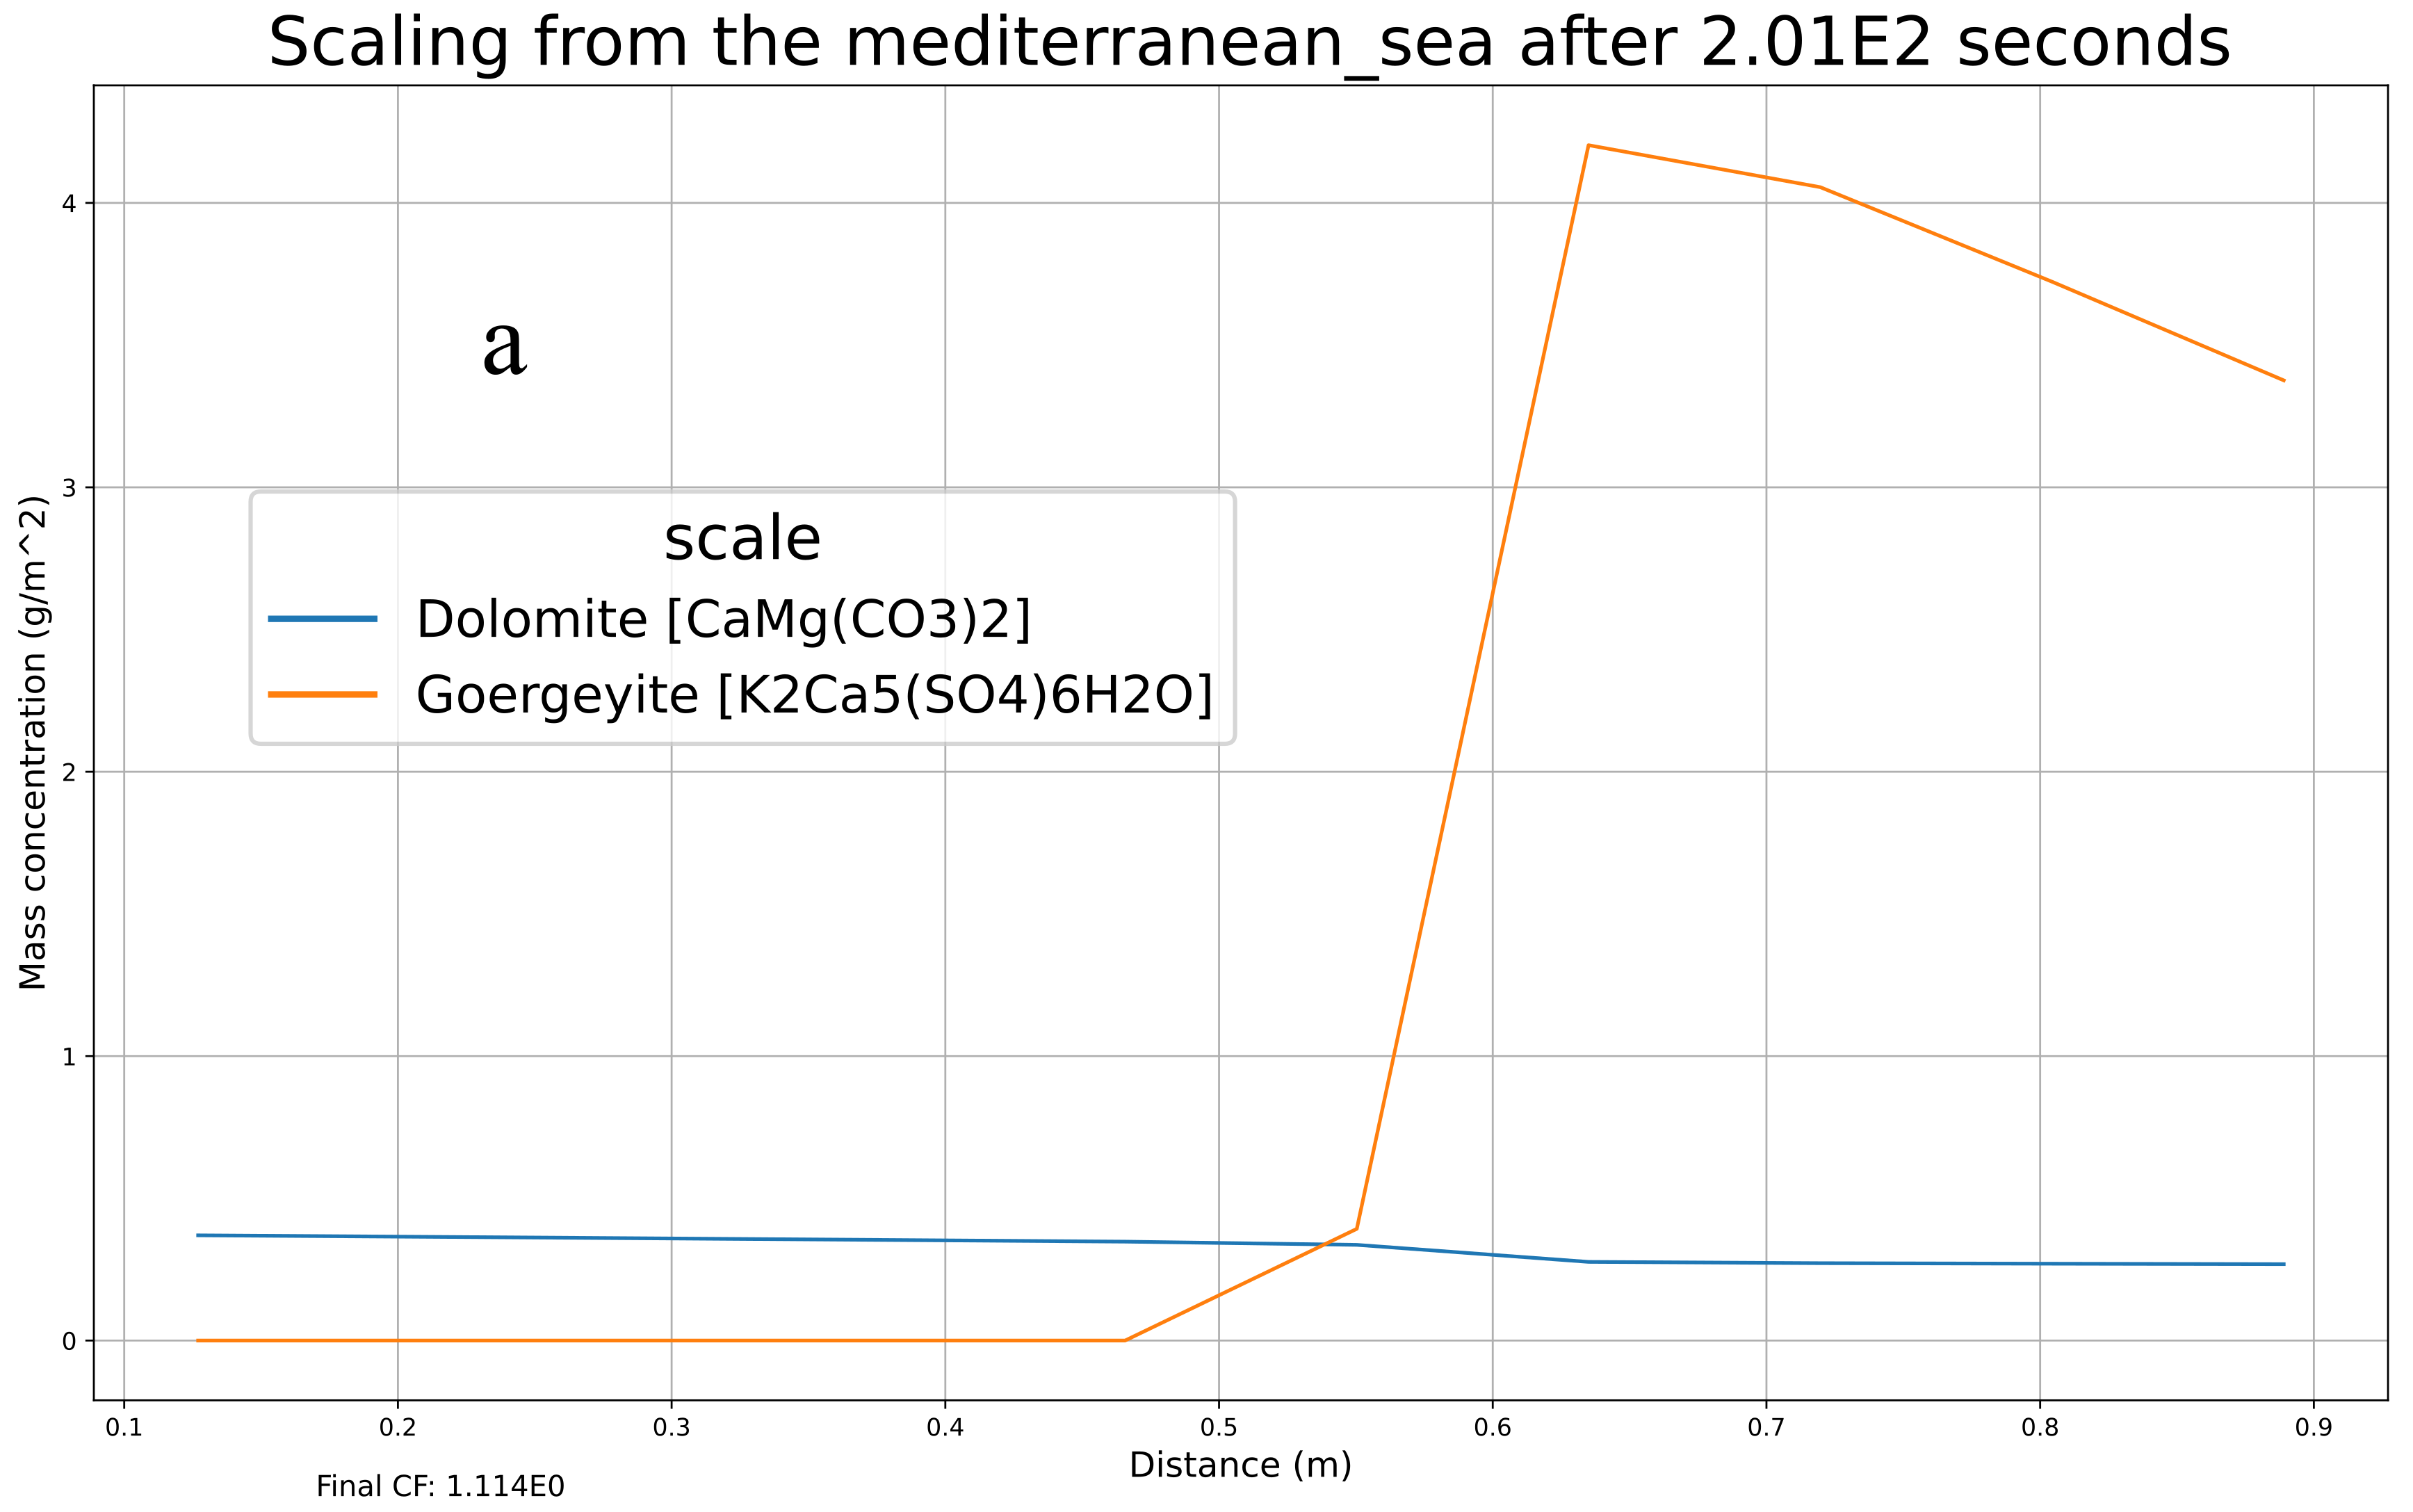
\includegraphics[width=0.49\textwidth]{images/ROSSpy/sensitivity_analyses/feed_source/Mediterranean.png} &
        \includegraphics[width=0.49\textwidth]{images/ROSSpy/sensitivity_analyses/feed_source/Palo_Duro_basin.png} \\ \midrule
        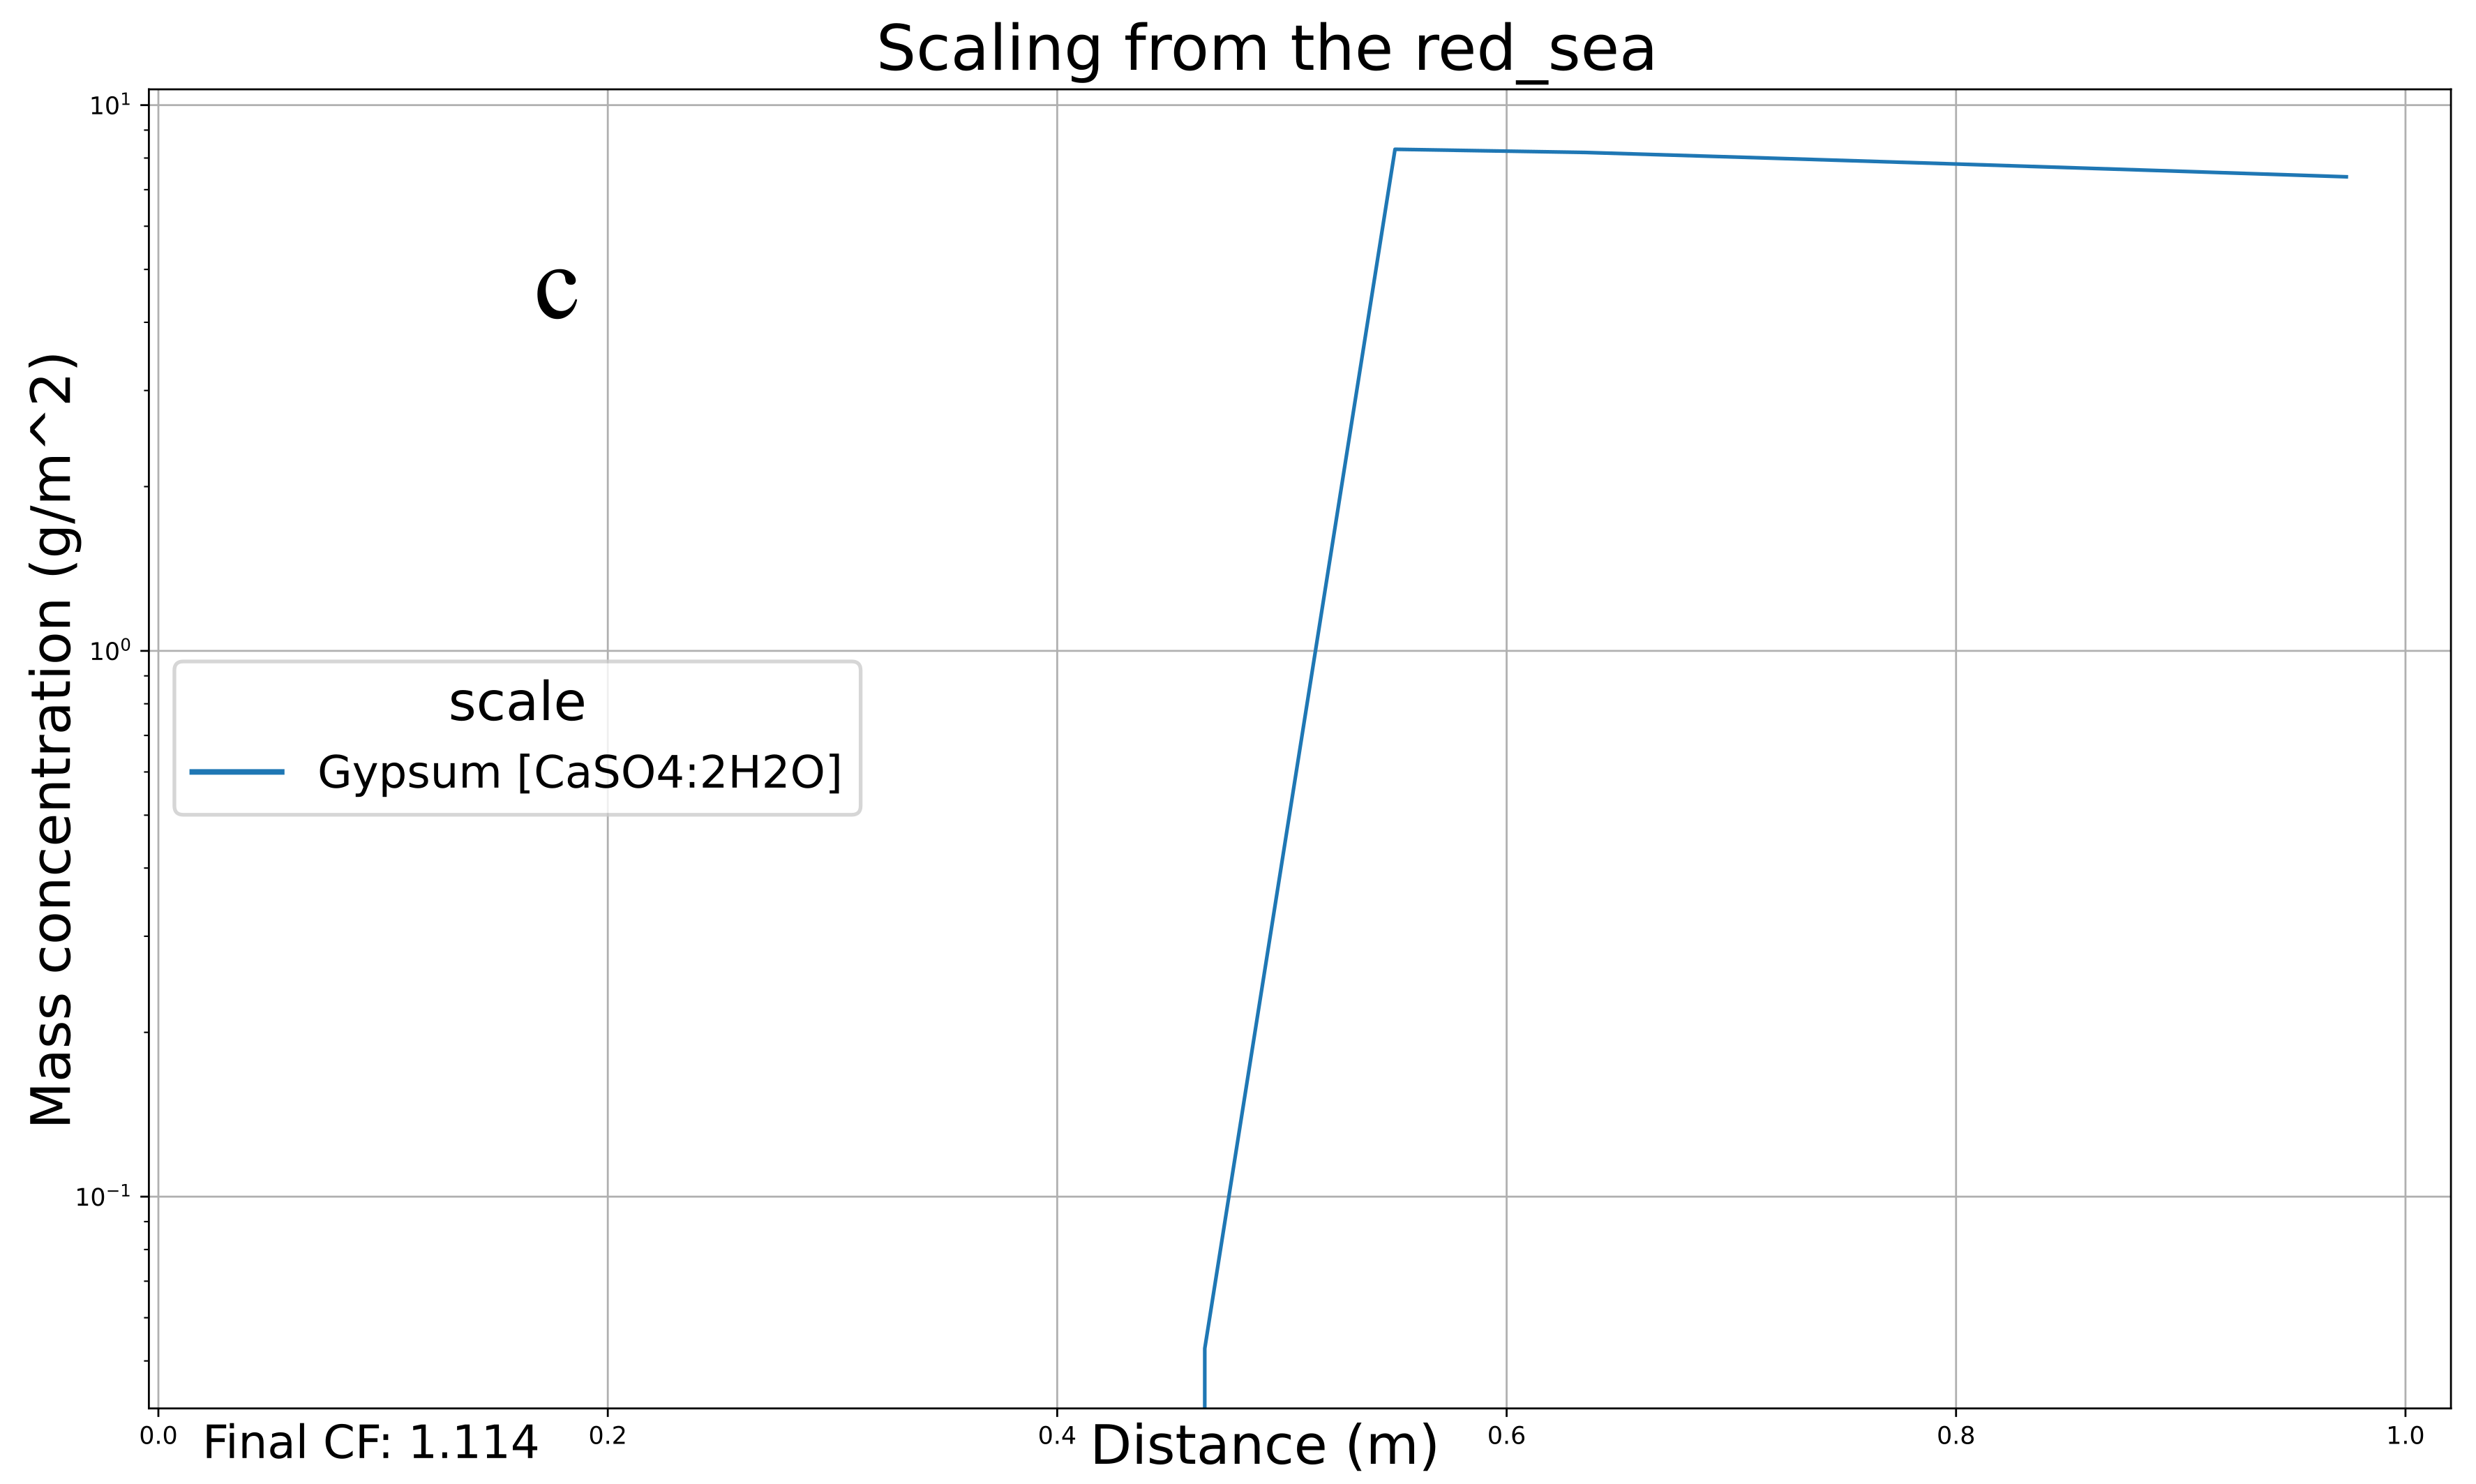
\includegraphics[width=0.49\textwidth]{images/ROSSpy/sensitivity_analyses/feed_source/Red_Sea.png} & 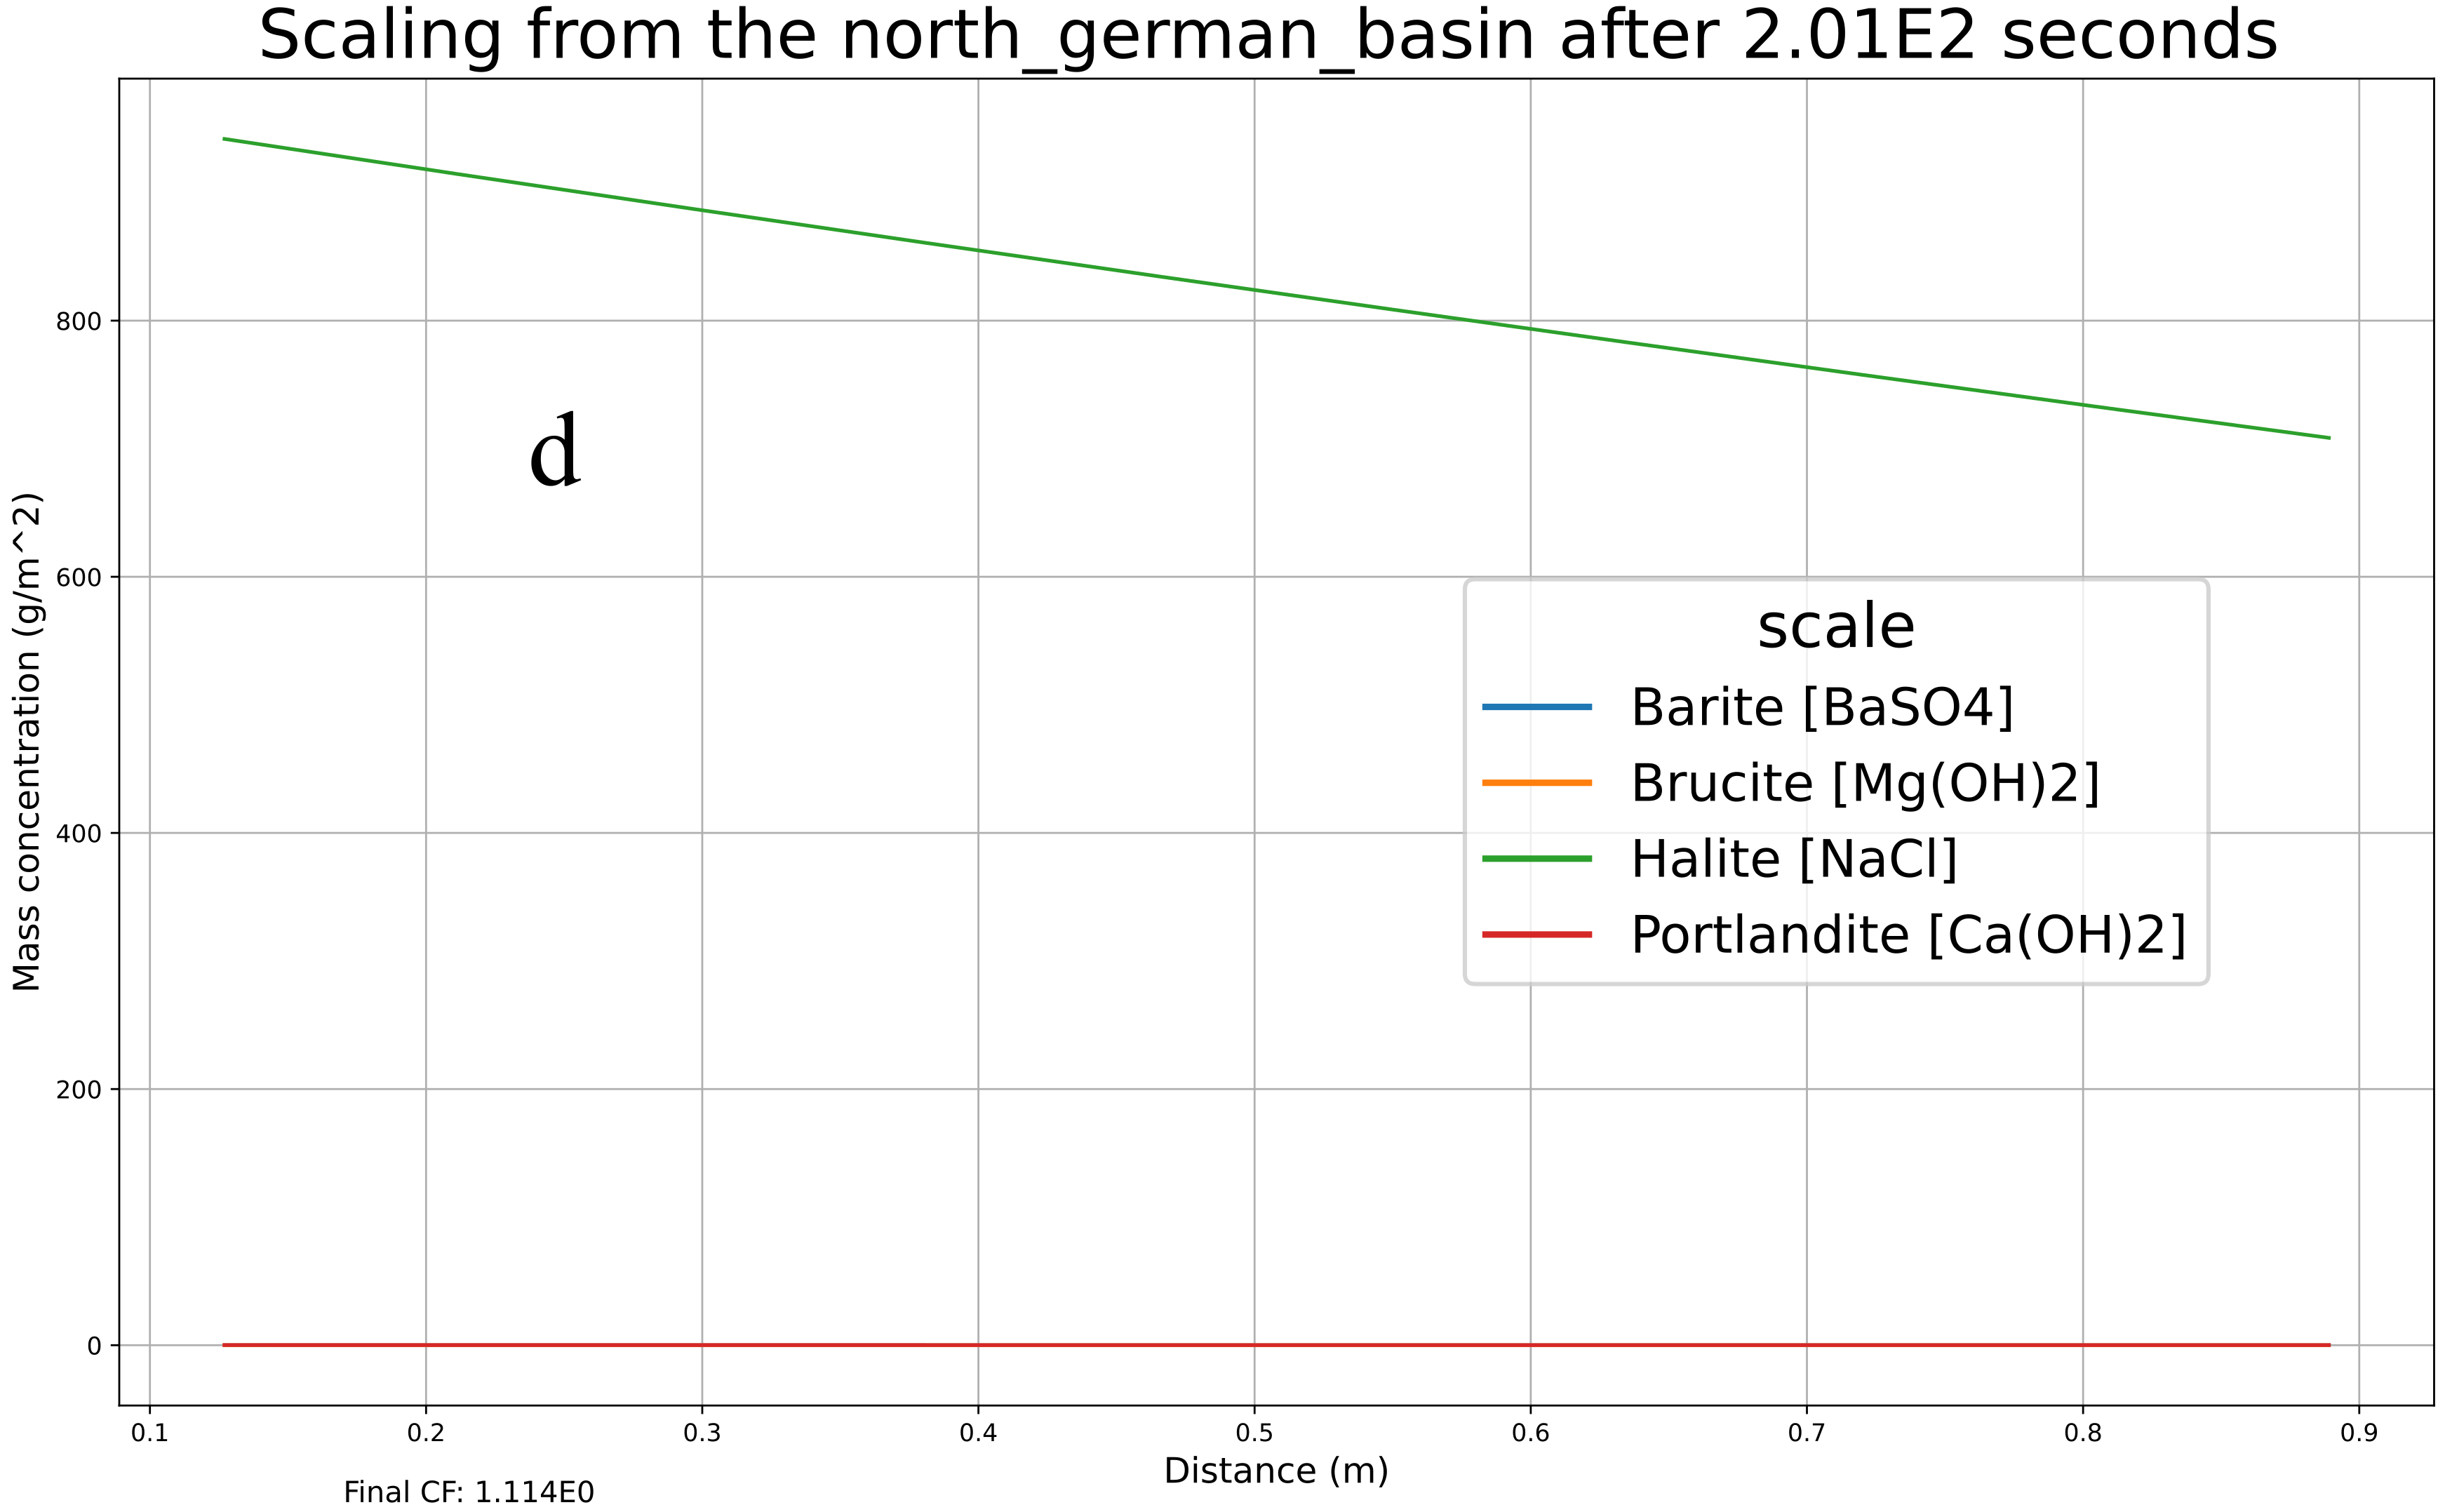
\includegraphics[width=0.49\textwidth]{images/ROSSpy/sensitivity_analyses/feed_source/German_Basin.png} \\ \bottomrule
    \end{tabular}
    \caption{
        Scaling predictions of a) the Mediterranean Sea, b) produced waters from the Palo Duro oil basin, c) the Red Sea, d) produced waters from the North German oil basin, with otherwise identical simulation parameters. These subfigures represent the spectrum of scaling predictions from the variety of different feed sources, which exhibits a high sensitivity of scale predictions to the feed geochemistry. 
    }
    \label{feed_sources}
\end{figure}

\section{Software}
ROSSpy, which is conceptualized by Figure \ref{workflow}, combines our one-dimensional RO model with post-processing operations that facilitate interpretation of the simulation results. The software a) translates parameters into a PHREEQ input file; b) executes that input file via PHREEQpy; c) processes the simulation results into figures and data tables via Matplotlib \cite{Hunter2007Matplotlib:Environment} and Pandas \cite{McKinney2011Pandas:Statistics} Python packages, respectively; and d) exports all of the simulation content -- e.g. the PHREEQ input file, SVG data figures, and CSV files of parameters, variables, data, and brine predictions -- into a specified folder and directory. The simulation data may be sliced into one-dimensional sets of distance or time that can be plotted against either scaling density or brine concentrations (Figures S2-S3) (see ROSSpy documentation).


\begin{figure}
    \centering
    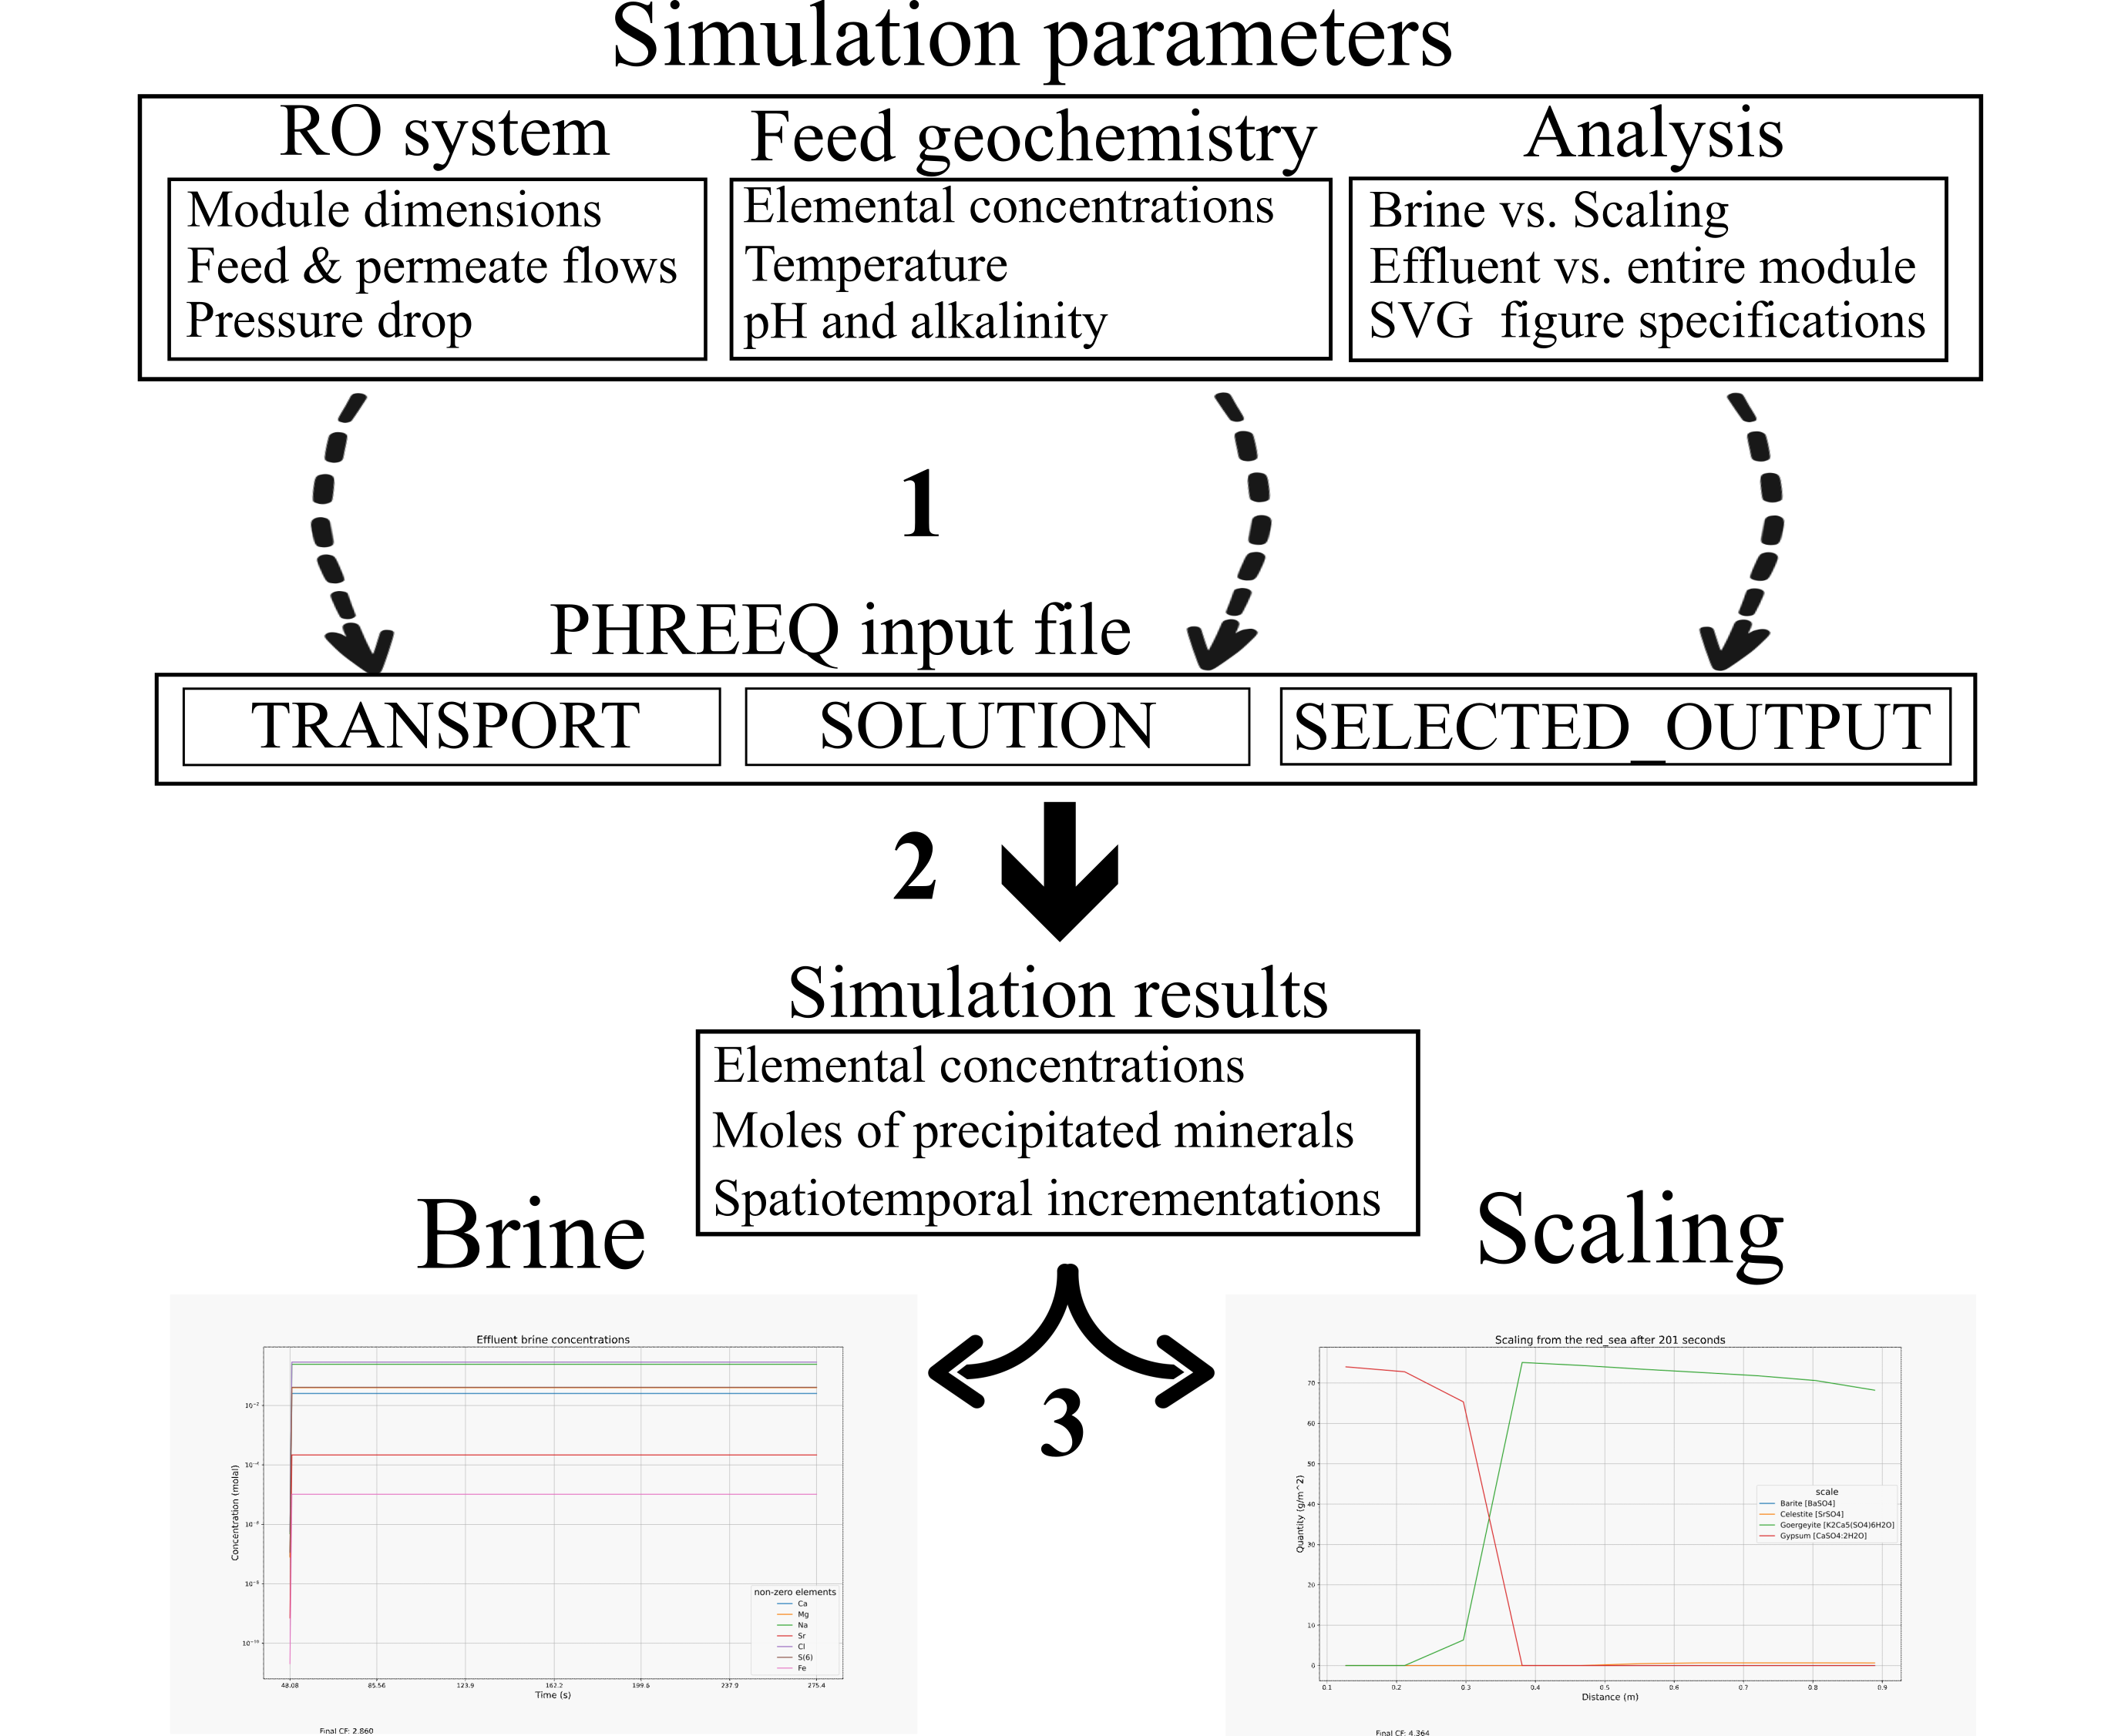
\includegraphics[width = \linewidth]{images/ROSSpy/rosspy_workflow_1.PNG}
    \caption{
        The ROSSpy workflow. Step 1 describes the translation of parameters -- i.e. module specifications, feed geochemistry, and simulation analysis -- into the corresponding code blocks of a PHREEQ input file. Step 2 describes executing the PHREEQ input file via either PHREEQpy in ROSSpy, or via the PHREEQC batch software in the interactive version of ROSSpy (iROSSpy) that is under development. Step 3 describes processing the predictions of brine concentrations or scaling quantities into representative figures and datatables, which are ultimately exported.
    }
    \label{workflow}
\end{figure}

\section{Conclusion}

A one-dimensional approximation of RO reactive transport geochemistry, executed in PHREEQC, is a practical and accurate representation of mineral scaling during desalination. The simulation predictions of this model were quantitatively and qualitatively verified for a few use cases, with both theoretical expectations and experimental data where it was available. The API implementation of this model (ROSSpy) furthermore meets identified needs of the community -- e.g. rapidly designing, executing, processing, and exporting simulations of RO scaling -- while maintaining accessibility through its light-weight design and its open-source code. We expect that this one-dimensional model and the unique attributes of ROSSpy  will facilitate scaling research and ultimately improve the efficiency of RO desalination towards alleviating chronic water insecurities in the world. 

\section{Funding}
This work was prepared in partial fulfillment of the requirements of the Berkeley Lab Undergraduate Research (BLUR) Program, managed by Workforce Development \& Education at the Berkeley Lab. The project was also partly funded by NSERC Discovery, MITACS Accelerate, CEWIL, and Canada Summer Jobs. 

% Acknowledgements section
\section{Acknowledgement}
The authors thank Ethan Sean Chan for his technical assistance in developing a graphical interface of ROSSpy (iROSSpy) that will be released in a future version. 